\documentclass[12pt, a4paper]{article}
\usepackage{graphicx} % Required for inserting images
\usepackage[final]{pdfpages}
\usepackage[serbian]{babel} % Use the Serbian language package
\usepackage{fontspec} % Required for using system fonts
\usepackage{geometry} % Required for setting page size
\usepackage{fancyhdr} % Required for custom headers and footers
\usepackage[scaled]{helvet}
\usepackage{csquotes}
\usepackage{chngcntr}
\usepackage[colorlinks=true,linkcolor=black,citecolor=black,urlcolor=black]{hyperref} % Customize link colors
\usepackage[fixlanguage]{babelbib} \bibliographystyle{babunsrt}
\usepackage{setspace}
\usepackage{tocloft}
\usepackage{minted} % Paket za umetanje koda
\usepackage{listings}
\usepackage{subcaption}
\usepackage{natbib}

% \setmainfont{Nimbus Sans L}
\setmainfont{Roboto}
\setlength{\parindent}{0pt}
\setlength{\parskip}{12pt}%

\geometry{a4paper, margin=1in}

% Customize headers and footers
\bibliographystyle{unsrtnat}


\counterwithin{figure}{section}
\addto\captionsserbian{\renewcommand{\figurename}{Слика}}

\setlength{\cftbeforesecskip}{1pt} % Razmak pre svake sekcije
\setlength{\cftparskip}{1pt} % Razmak između stavki u sadržaju

\definecolor{codegreen}{rgb}{0,0.6,0}
\definecolor{codegray}{rgb}{0.5,0.5,0.5}
\definecolor{codepurple}{rgb}{0.58,0,0.82}
\definecolor{backcolour}{rgb}{0.95,0.95,0.92}

\setminted{style=xcode}


\begin{document}

\lstdefinestyle{mystyle}{
    backgroundcolor=\color{backcolour},   
    commentstyle=\color{codegreen},
    keywordstyle=\color{magenta},
    numberstyle=\tiny\color{codegray},
    stringstyle=\color{codepurple},
    basicstyle=\ttfamily\footnotesize,
    breakatwhitespace=false,         
    breaklines=true,                 
    captionpos=b,                    
    keepspaces=true,                 
    numbers=left,                    
    numbersep=5pt,                  
    showspaces=false,                
    showstringspaces=false,
    showtabs=false,                  
    tabsize=2
}



\includepdf[pages=-]{prva_strana.pdf}

\renewcommand{\contentsname}{Садржај} % Change the name of the Table of Contents
\addtocontents{toc}{\protect\thispagestyle{empty}}
\tableofcontents % Print the Table of Contents
\clearpage % Start a new page
\setcounter{page}{3}
\pagestyle{fancy}
\fancyhf{} % Clear header and footer
\fancyfoot[R]{\thepage} % Right align page number in the footer
\renewcommand{\headrule}{} % Remove header line

\section{Увод}
\textit{Blockchain} технологија представља дистрибутивну, децентрализовану и јавну базу свих трансакција \cite{1}.


Први концепт \textit{blockchain} технологије помиње се у 1982. години, када је Давид Чаум у својој дисертацији описао дистрибуирану базу података која користи криптографију \cite{2}. Овај рани рад није био директно повезан са дигиталним валутама, али је поставио темеље за будући развој \textit{blockchain} - а.

Права револуција долази 2008. године када Сатоши Накамото објављује рад "\textit{Bitcoin}: \textit{Peer-to-peer} електронски готовински систем", уводећи први модерни \textit{blockchain} и криптовалуту \textit{Bitcoin}. Генесис блок, први блок \textit{Bitcoin blockchain} - а, ископан је 3. јануара 2009. године, означавајући почетак \textit{blockchain} технологије какву данас познајемо \cite{3}.

\textit{Etherium}, лансиран 2015. године од стране Виталика Бутерина, увео је паметне уговоре који омогућавају сложеније трансакције и аутоматизацију различитих процеса. Овај развој проширио је примену \textit{blockchain} технологије далеко изван дигиталних валута, омогућавајући креирање децентрализованих апликација \cite{4}.

\textit{Blockchain} технологије су се од свог настанка имплементирале у различитим програмским језицима и окружењима. У својим раним фазама, \textit{blockchain} технологије су се углавном развијале користећи језике као што су \textit{C++} и \textit{Java}, захваљујући њиховој ефикасности и широкој употреби у индустрији. Касније, с појавом паметних уговора, \textit{Solidity} је постао стандард за развој на \textit{Etherium} платформи.

Овај рад се фокусира на имплементацију основних концепата \textit{blockchain} технологије у програмском језику \textit{Rust}, који је познат по својој сигурности, перформансама и могућности превенције грешака при руковању меморијом.

Рад је структуиран у шест целина. Прва целина бавиће се основама \textit{Rust} програмског језика, којим је имплементиран концепт пројекта. Друга целина се односи на увод у \textit{blockchain} технологију. Детаљи треће целине односе се на архитектуру \textit{blockchain} мреже, као што су блокови, ланац, новчаник, трансакције итд. Четврта целина разрађује клијенте у \textit{blockchain} мрежи. У претпоследњем поглављу објашњене су могуће тачке проширења решања и теме за даља истраживања. Последње поглавље је закључак рада.
\pagebreak

\section{Основе \textit{Rust} програмског језика}
\textit{Rust} је савремени програмски језик који је развијен да буде безбедан и брз. Развијен од стране \textit{Mozilla Research}-а, \textit{Rust} је од свог настанка привукао велику пажњу због својих изузетних безбедносних карактеристика и перформанси \cite{5}.

\subsection{Увод у \textit{Rust} програмски језик}
\textit{Rust} је системски програмски језик, а уместо интерпретираног језика, као што су \textit{JavaScript} или \textit{Ruby}, има компајлер, као што имају \textit{Go}, \textit{C} или \textit{Swift}. Не комбинује активни \textit{runtime}, али обезбеђује језичку ергономију. Све је ово могуће захваљујући компајлеру који спречава грешке било којег типа и осигурава да не дође до проблема у меморији пре него што се покрене апликација \cite{6}.

\textit{Rust} обезбеђује перформансе (нема \textit{runtime}, нити прикупљање "смећа"), безбедност (компајлер осигурава да је све безбедно за меморију, чак и у асинхроним окружењима) и продуктивност (његове уграђене алатке за тестирање, документацију и "менаџер" пакета чине га лаким за израдз и одржавање) \cite{6}. 

\subsection{Зашто \textit{Rust} за \textit{blockchain}?}
Када је у питању развој blockchain апликација, \textit{Rust} се истиче као одличан избор из неколико разлога:
\begin{enumerate}
    \item \textbf{Безбедност меморије}: \textit{Rust}-ов систем власништва и провера за време компилације осигуравају да програмери избегну уобичајене грешке у раду са меморијом, што је критично за сигурност \textit{blockchain} система \cite{7}.
    \item \textbf{Перформансе}: \textit{Rust} је дизајниран да буде брз и ефикасан. Његов минималан \textit{overhead} и високо оптимизован компајлер резултирају брзим извршавањем кода, што је важно за обраду великог броја трансакција у реалном времену \cite{7}.
    \item \textbf{Паралелизам и конкурентност}: \textit{Rust} нуди снажну подршку за паралелно и конкурентно програмирање, омогућавајући оптимално коришћење мулти-језгарних процесора \cite{7}.
\end{enumerate}

\textit{Rust} нуди низ алата и библиотека које олакшавају развој сложених апликација. Две од најзначајнијих библиотека за развој \textit{blockchain} апликација су \textit{Tokio} и \textit{libp2p}. Ове библиотеке пружају подршку за асинхроне позиве и \textit{peer-to-peer} комуникацију, што је кључно за функционалност и ефикасност \textit{blockchain} система.

\pagebreak

% \textbf{\textit{Tokio}} је моћна асинхрона \textit{runtime} библиотека за \textit{Rust} која омогућава развој високоперформансних и високо доступних апликација. Кроз \textit{Tokio}, програмери могу да имплементирају асинхроне позиве и да развију веб сервере који могу да обрађују велики број истовремених веза.

Слика \ref{fig:2.1} прииказује технички стек који је укључен у одабир радног оквира. \textbf{\textit{Warp}} је довољно мали да се "склони са пута", довољно се користи да се њиме управља активно и има активну заједницу. Заснован је на \textit{Tokio runtime} - у. 


\begin{figure}[h]
    \centering
    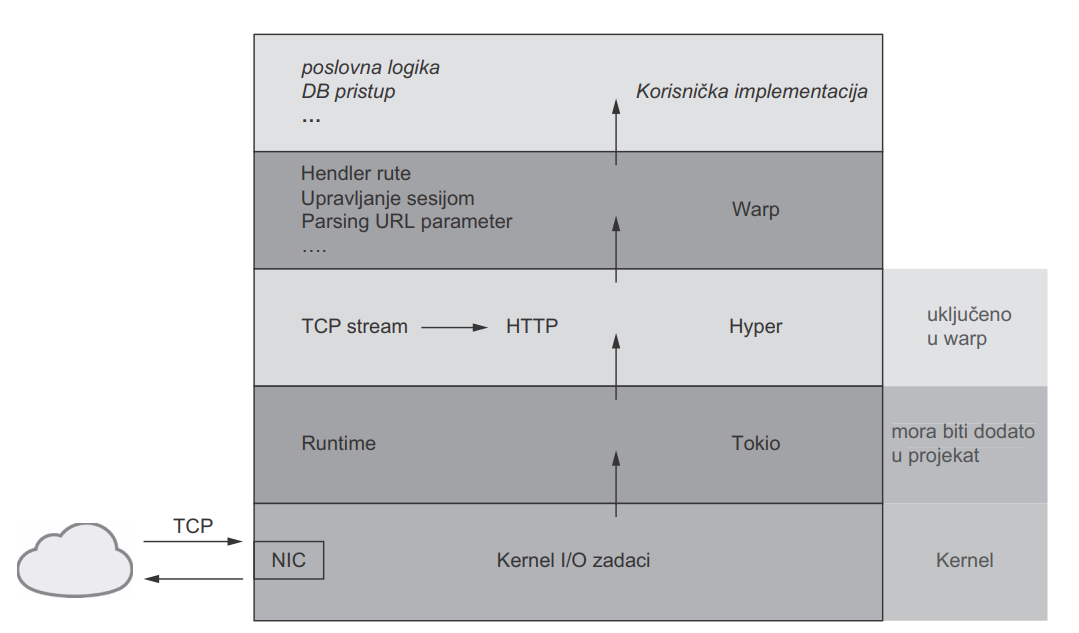
\includegraphics[width=1\linewidth]{slike/warp.png}
    \caption{\textit{Warp} веб радни оквир}
    \label{fig:2.1}
\end{figure}

\textit{\textbf{libp2p}} је модуларни мрежни стек који омогућава \textit{peer-to-peer} комуникацију. У контексту \textit{blockchain}-а, \textit{libp2p} се користи за омогућавање комуникације између различитих чворова у мрежи. Ова библиотека је флексибилна и подржава различите протоколе за пренос података, што је чини идеалном за развој децентрализованих апликација.

\pagebreak

\section{Увод у \textit{blockchain} технологију}
\textit{Blockchain} технологија представља савремен приступ складиштењу и дистрибуцији података. Основни принципи и концепти \textit{blockchain} технологије нуде дубоку промену у начину на који се информације похрањују, проверавају и дистрибуирају путем децентрализоване мреже рачунара.

\subsection{Основни принципи и концепти}
\textit{Blockchain} се може дефинисати као дистрибуисана дигитална књига трансакција. Основна идеја је стварање низа блокова који садрже податке. Блкови су криптографски повезани тако да је немогуће мењати податке у претходним блоковима без мењања свих следећих блокова \cite{8}. 

Кључни елементи \textit{blockchain}-а укључују:
\begin{enumerate}
    \item \textbf{Децентрализација}: Подаци се похрањују и управљају путем мреже чворова уместо централизованог ауторитета, што осигурава транспарентност и отпорност на цензуру.
    \item  \textbf{Дистрибуираност}: Сваки чвор у мрежи садржи комплетан или део \textit{blockchain}-а, омогућујући свима у мрежи да виде исте податке. Ово спречава појединачне тачке квара и повећава отпорност на нападе.
    \item \textbf{Сигурност}: Криптографски алгоритми осигуравају да је свака промена у \textit{blockchain}-у лако проверљива, а трансакције се потврђују кроз консензус мреже.
    \item \textbf{Неповратност}: Након што је трансакција забележена у \textit{blockchain}-у, тешко ју је променити или обрисати без сагласности већине чворова у мрежи, чиме се осигурава поверење и интегритет података.
\end{enumerate}


\subsection{Поређење са традиционалним базама података}
Насупрот традиционалним базама података које су често централизоване и ослањају се на поверење у једну јединицу, \textit{blockchain} нуди неколико кључних разлика \cite{9}:
\begin{enumerate}
    \item \textbf{Централизација у односу на децентрализацију}: Традиционалне базе података често су централизоване под контролом једне организације. \textit{Blockchain} дистрибуише податке широм мреже, елиминишући потребу за централним ауторитетом.
    \item \textbf{Транспарентност и проверљивост}: \textit{Blockchain} омогућава свим корисницима увид у све трансакције које су се догодиле, што повећава транспарентност и смањује могућност манипулације.
    \item \textbf{Сигурност и отпорност}: Због своје дистрибуиране природе, \textit{blockchain} је отпорнији на нападе и кварове у поређењу са традиционалним базама података које су осетљиве на појединачне тачке квара.
    \item \textbf{Ефикасност и трошкови}: Иако \textit{blockchain} може бити спорији у обради података у поређењу са централизованим базама података, његова сигурност и транспарентност могу надмашити трошкове и ризике традиционалних система.
\end{enumerate}

\newpage
\section{Архитектура \textit{blockchain} мреже}
\textit{Blockchain} технологија се састоји од неколико кључних компоненти које омогућавају њено функционисање. Основне јединице података су блокови, који садрже информације о трансакцијама, временским ознакама и криптографским хеш функцијама претходних блокова. Ови блокови су повезани у секвенцијални ланац, познат као \textit{blockchain}, који осигурава неповредивост података. 

Дистрибуирана мрежа чворова заједнички одржава и верификује \textit{blockchain}, омогућавајући децентрализацију. Консензус алгоритми, као што су \textit{Proof of Work (PoW)} и \textit{Proof of Stake (PoS)}, омогућавају учесницима мреже да се сложе око валидности нових блокова \cite{10}. Криптографија осигурава сигурност и приватност података унутар \textit{blockchain} -а, користећи хеш функције и дигиталне потписе. 

У наредним подсекцијама, детаљно ћемо описати сваку од ових компоненти, укључујући процесе као што су \textit{PoW} и \textit{mining}, који су кључни за додавање нових блокова у ланац.


\subsection{Блокови}
Блокови су основне јединице података у \textit{blockchain} технологији. Сваки блок садржи скуп података који су повезани са трансакцијама и другим важним информацијама. У контексту \textit{blockchain}-а, блокови су организовани у ланац, где сваки блок садржи хеш претходног блока, што обезбеђује интегритет и сигурност података. Следећи код приказује структуру блока у Rust програмском језику:

\begin{minted}{rust}
pub struct Block {
    pub timestamp: DateTime<Utc>,
    pub last_hash: String,
    pub hash: String,
    pub data: Vec<Transaction>,
    pub nonce: u64,
    pub difficulty: u64,
}
\end{minted}

Атрибути блока су:
\begin{itemize}
    \item \textbf{\textit{timestamp}}: Време када је блок креиран. Овај атрибут омогућава праћење хронологије трансакција у \textit{blockchain}-у.
    \item \textbf{\textit{last\_hash}}: Хеш вредност претходног блока у ланцу. Овај атрибут обезбеђује да сваки блок буде повезан са својим претходником, чиме се осигурава интегритет ланца.
    \item \textbf{\textit{hash}}: Хеш вредност тренутног блока. Ова вредност се добија применом хеш функције на садржај блока и служи као јединствени идентификатор блока.
    \item \textbf{\textit{data}}: Податке у блоку, који обично укључују трансакције. У овом случају, то је вектор трансакција \textit{(Vec<Transaction>)}.
    \item \textbf{\textit{nonce}}: Произвољни број који рудари мењају током процеса рударења како би добили хеш вредност блока која задовољава критеријуме тешкоће.
    \item \textbf{\textit{difficulty}}: Ниво тежине који одређује колико је сложено пронаћи важећи хеш за блок. Тежина рударења се прилагођава да би се одржала константна брзина креирања блокова у мрежи.
\end{itemize}



\subsubsection{Генесис блок}
Генесис блок је први блок у ланцу блокова и служи као темељ целокупног \textit{blockchain} система (Слика \ref{fig:genesis-block}) \cite{8}. Он нема претходника и обично је ручно креиран од стране креатора \textit{blockchain}-а. Генесис блок обично садржи посебне параметре и почетне вредности које су специфичне за дат \textit{blockchain}. Његова важност лежи у чињеници да сваки наредни блок у ланцу зависи од њега кроз хеш вредности.

\begin{figure}[h]
    \centering
    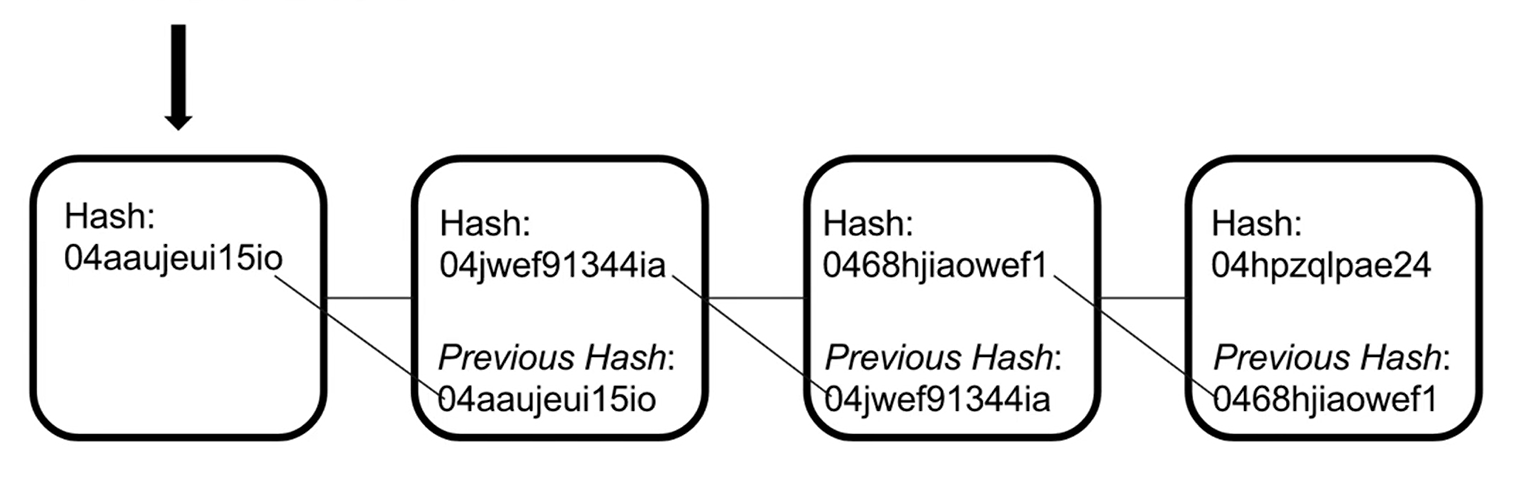
\includegraphics[width=1\linewidth]{slike/genesis.png}
    \caption{Приказ генесис блока у \textit{blockchain}-у}
    \label{fig:genesis-block}
\end{figure}

\subsubsection{Рударење}
Рударење је процес додавања нових блокова у \textit{blockchain}. Рудари користе своју рачунарску снагу да реше комплексне математичке проблеме који су потребни за валидацију нових трансакција и креирање нових блокова. Овај процес захтева значајну количину енергије и ресурса, али је кључан за одржавање безбедности и децентрализације \textit{blockchain} мреже. У процесу рударења, рудари се такмиче да пронађу одговарајући \textit{nonce} који ће произвести хеш вредност која испуњава одређене критеријуме тешкоће.


\subsubsection{Хеш функција}
Хеш функција је критичан елемент у \textit{blockchain} технологији, јер обезбеђује сигурност и интегритет података у блоковима. Хеш функција узима улазне податке произвољне дужине и генерише фиксну дужину излазне вредности, која је јединствена за те улазне податке. У контексту \textit{blockchain}-а, хеш функција се користи да повезује сваки блок са претходним блоком, чиме се обезбеђује да свака промена у подацима било ког блока одмах утиче на све наредне блокове, што чини \textit{blockchain} изузетно отпорним на манипулацију.



\subsection{Ланац}
\textit{Blockchain} је структура података која се састоји од низа повезаних блокова, где сваки блок садржи хеш претходног блока, чиме се обезбеђује интегритет и сигурност ланца. Следећи код приказује структуру \textit{blockchain}-а у \textit{Rust} програмском језику:

\begin{minted}{rust}
pub struct Blockchain {
    pub chain: Vec<Block>,
}
\end{minted}

Атрибут \textit{\textbf{chain}} је вектор који чува редоследно повезане блокове, формирајући ланац блокова.
Слика \ref{fig:genesis-blockchain} приказује структуру ланца са генесис блоком на почетку.
\begin{figure}[h]
    \centering
    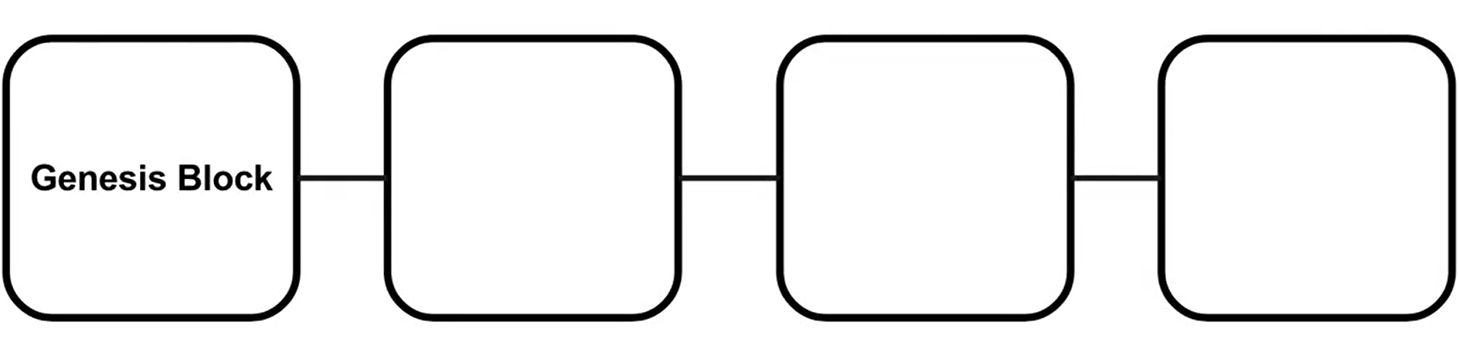
\includegraphics[width=1\linewidth]{slike/blockchain.png}
    \caption{Приказ идеје \textit{blockchain}-a}
    \label{fig:genesis-blockchain}
\end{figure}

\newpage
\subsubsection{Валидација више ланаца}
Идеја овог механизма је да подржи више доприносиоца, при чему ће више доприносиоца додавати блокове у \textit{blockchain}. Сваки рудар ће имати своју верзију истог ланца. Када један рудар дода нови блок у ланац, мораће да пошаље тај нови блок осталим ланцима у систему како би они прихватили ту промену и ажурирали целокупни систем. На тај начин сви добијају ажурирану копију са тим новим блоком, чиме се осигурава да сви ланци буду конзистентни.


\begin{figure}[h]
    \centering
    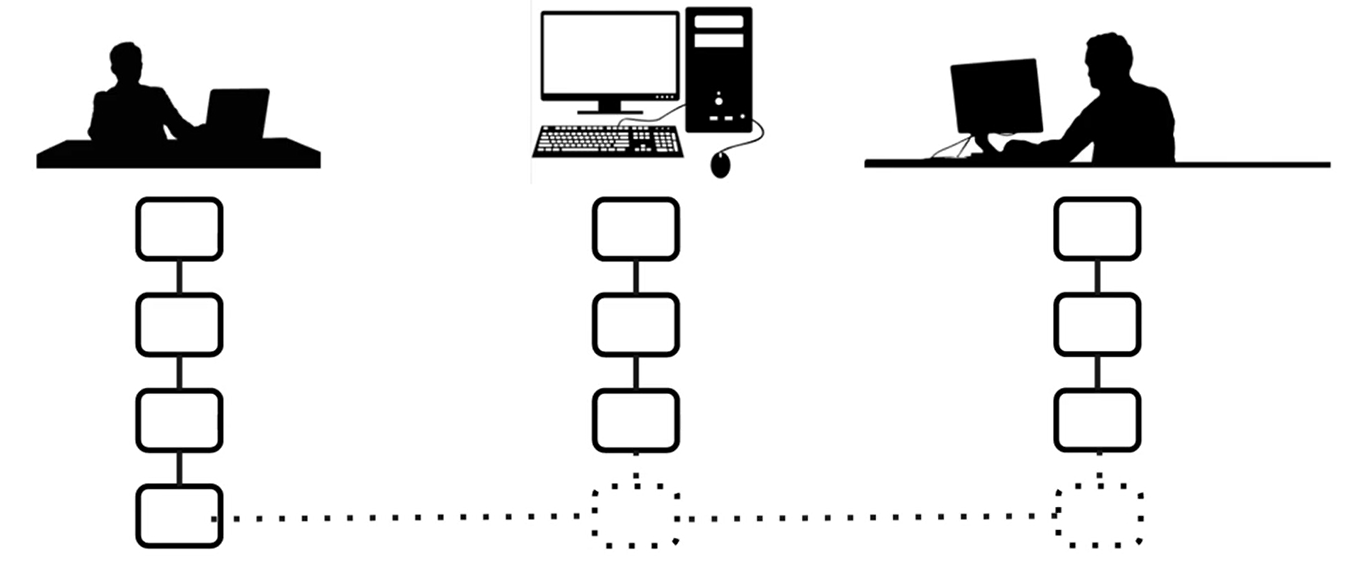
\includegraphics[width=1\linewidth]{slike/multiple-chain-validation.png}
    \caption{Приказ дељења ланаца}
    \label{fig:multiple-chain-validation}
\end{figure}

Међутим, да би сви рудари прихватили ове нове ланце, мора постојати неки облик валидације који ће осигурати да је нови блок валидан и да треба да буде прихваћен. Главни облик валидације је прихватање дужих ланаца који стигну. На пример, ако сви имају договорени \textit{blockchain} који је већ дуг три блока, и један рудар дода два блока у ланац, док други рудар дода само један блок у исто време, систем ће прихватити дужи ланац. На тај начин се осигурава да договорени ланац за све увек буде онај који садржи највише података.


\begin{figure}[h]
    \centering
    \begin{minipage}{0.45\linewidth}
        \centering
        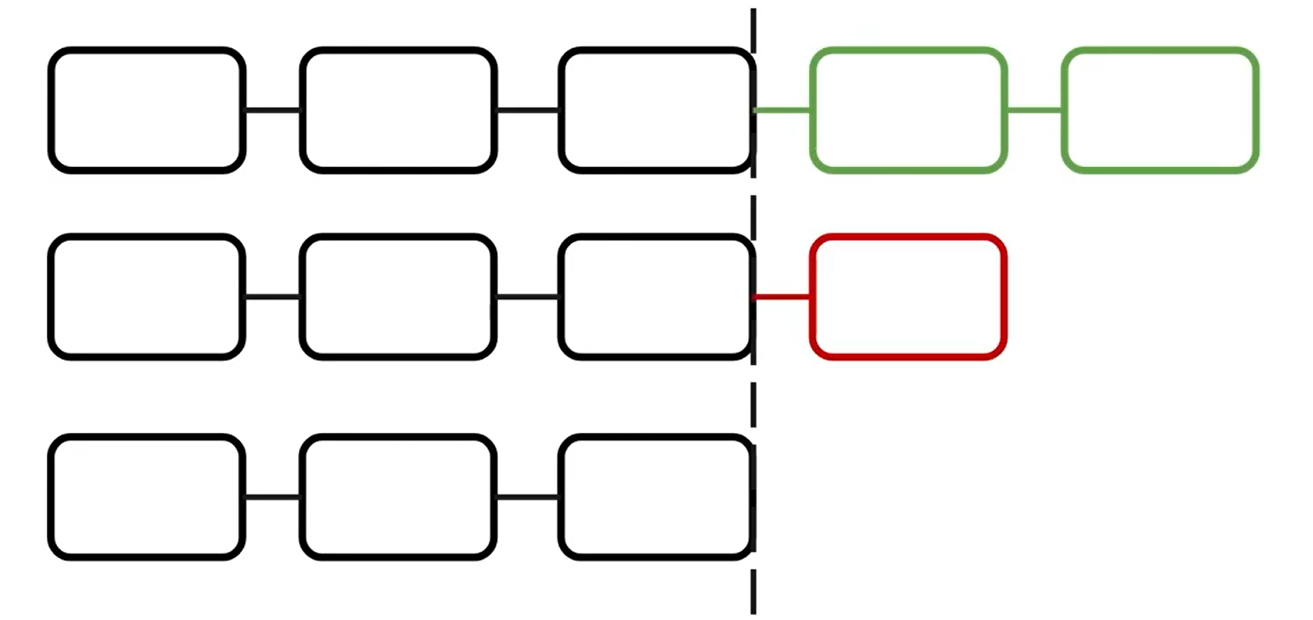
\includegraphics[width=\linewidth]{slike/longer-chains-before.png}
        \caption{Стање пре валидације}
        \label{fig:validation-1}
    \end{minipage}
    \hfill
    \begin{minipage}{0.45\linewidth}
        \centering
        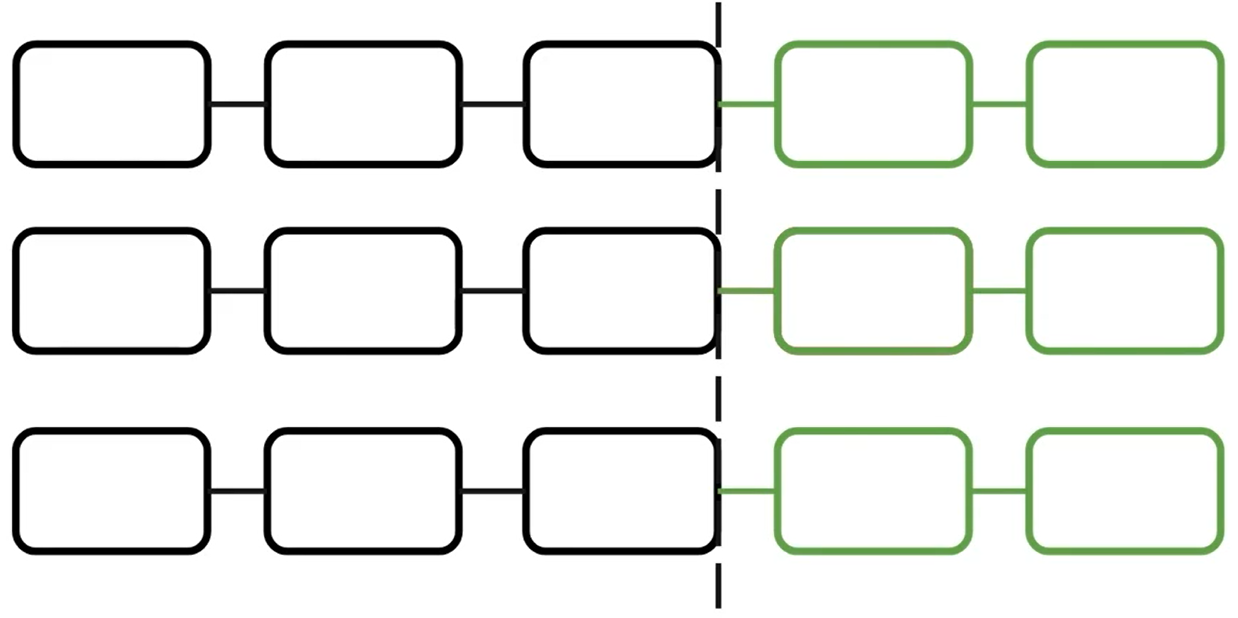
\includegraphics[width=\linewidth]{slike/longer-chains-after.png}
        \caption{Стање после валидације}
        \label{fig:validation-2}
    \end{minipage}
\end{figure}

\newpage
Ово такође решава проблем рачвања у ланцу. На пример, ако две одвојене инстанце \textit{blockchain}-а истовремено произведу један блок на основу претходног блока, настаје рачвање у систему где оба рудара производе блок на основу истог претходног блока (слика \ref{fig:forks-a}). Пола рудара ће имати ланац који је произвео рудар А, а друга половина ће имати ланац који је произвео рудар Б (слика \ref{fig:forks-b}). Коначно, систем треба да дође до договора о томе који ланац ће прихватити. Ако неко дода неколико блокова на ланац рудара А, тај ланац ће сада бити дужи од свих осталих у систему (слика \ref{fig:forks-c}). Сви ће морати да прихвате најдужи ланац, који садржи блок од рудара А, чиме се решава рачвање прихватањем оригиналног блока од рудара А (слика \ref{fig:forks-d}).

\begin{figure}[h]
    \centering
    \begin{subfigure}{0.45\linewidth}
        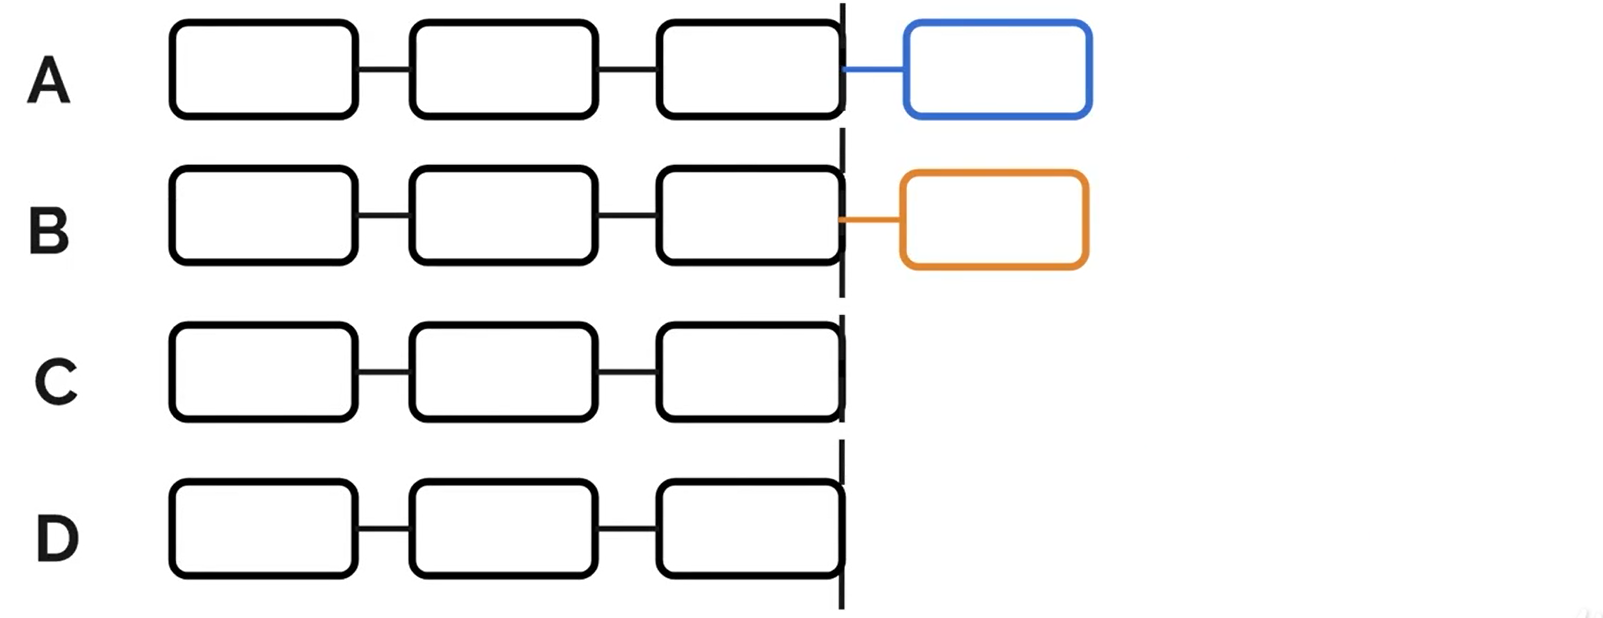
\includegraphics[width=\linewidth]{slike/forks-1.png}
        \caption{Додавање различитих блокова}
        \label{fig:forks-a}
    \end{subfigure}
    \hfill
    \begin{subfigure}{0.45\linewidth}
        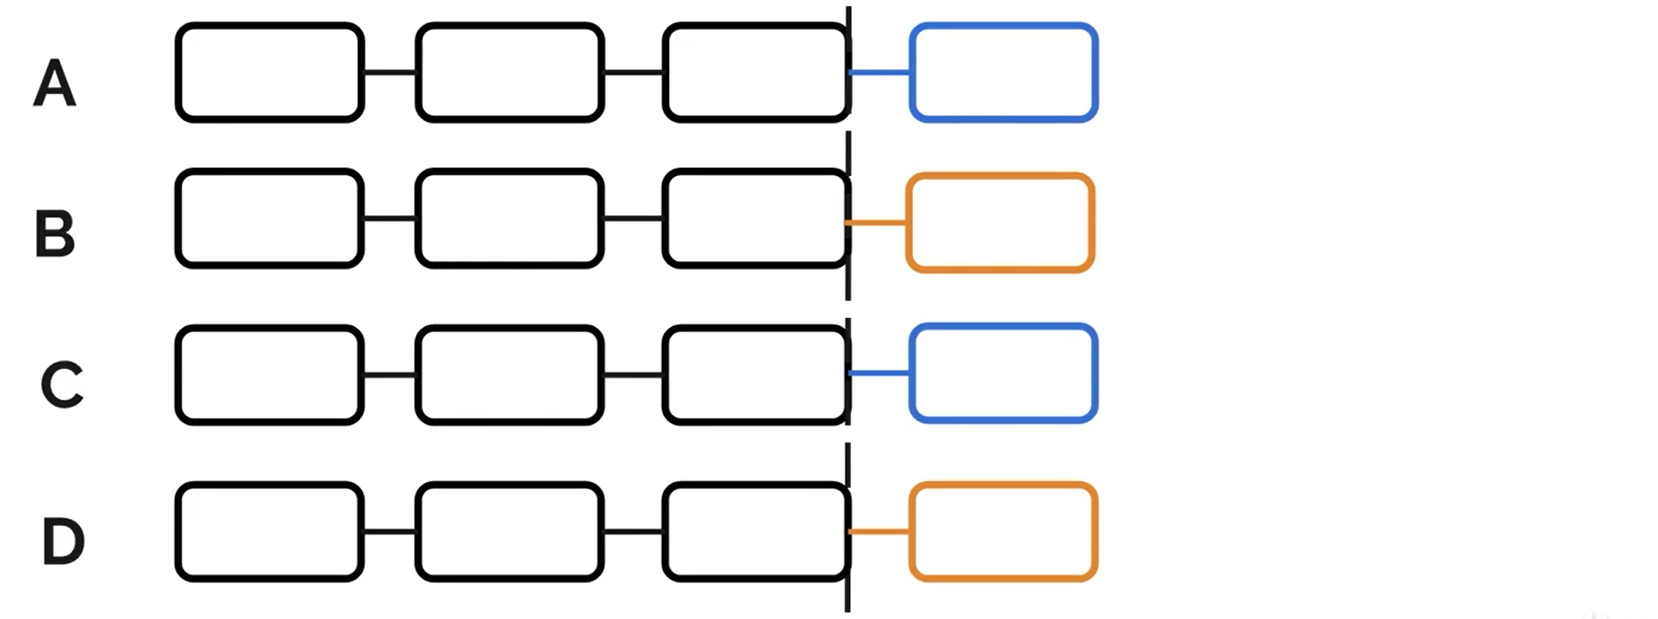
\includegraphics[width=\linewidth]{slike/forks-2.png}
        \caption{Размена различитих ланаца}
        \label{fig:forks-b}
    \end{subfigure}

    \begin{subfigure}{0.45\linewidth}
        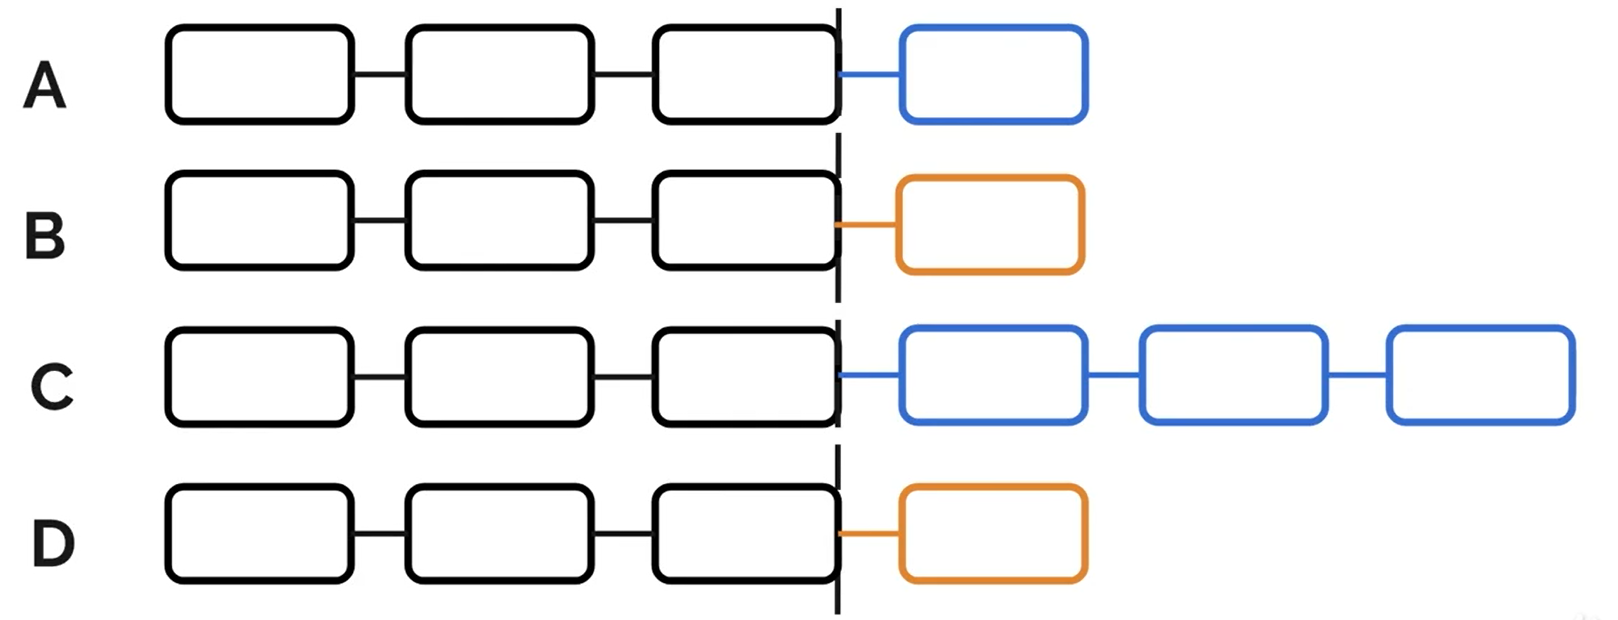
\includegraphics[width=\linewidth]{slike/forks-3.png}
        \caption{Додавање нових блокова}
        \label{fig:forks-c}
    \end{subfigure}
    \hfill
    \begin{subfigure}{0.45\linewidth}
        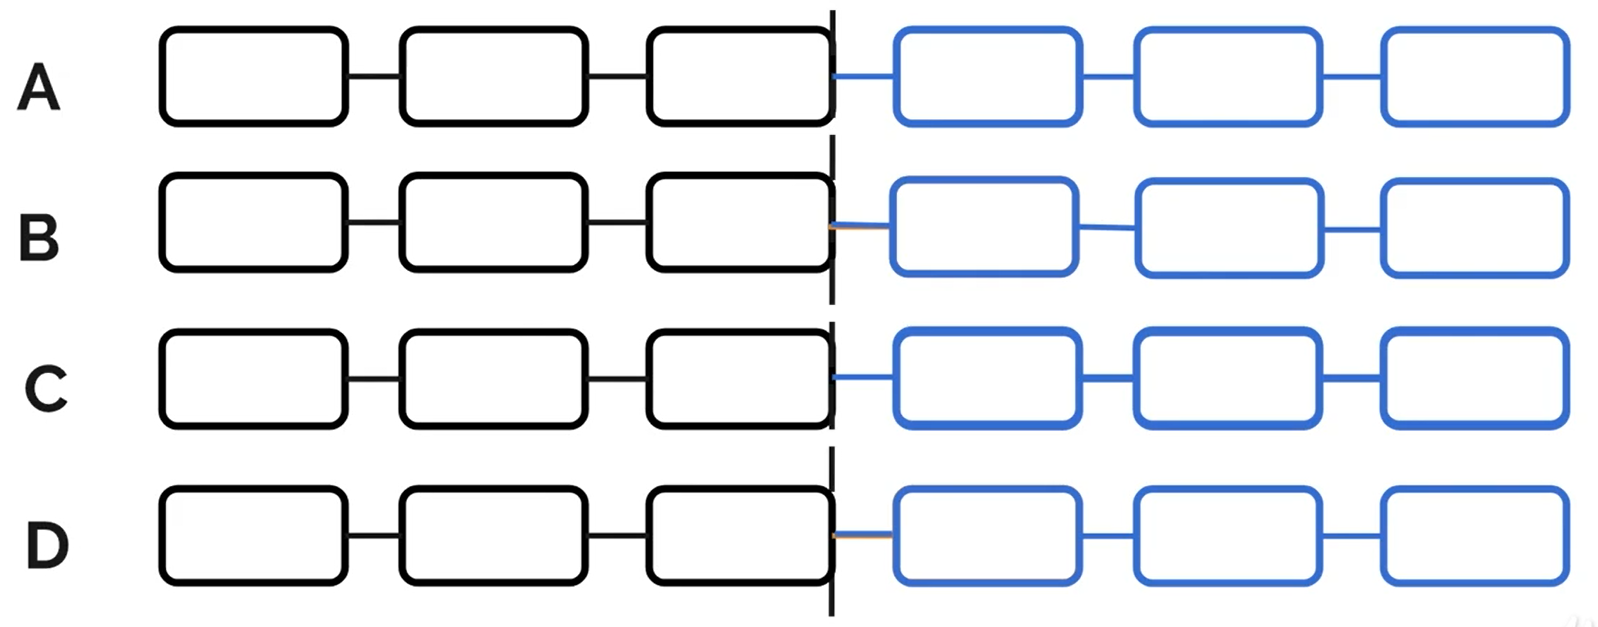
\includegraphics[width=\linewidth]{slike/forks-4.png}
        \caption{Прихватање најдужег ланца}
        \label{fig:forks-d}
    \end{subfigure}
    \caption{Решавање рачвања}
    \label{fig:combined}
\end{figure}

Ово не значи да блокови са ланца рудара Б губе оригиналне податке, јер се блок који није укључен у рачвање може сада додати на крај новоприхваћеног ланца.

Други облик валидације је провера вредности хеша произведених за сваки блок ланца. Сваки \textit{blockchain} има приступ хеш функцији која генерише хеш на основу података блока. Када \textit{blockchain} прими нови ланац, може осигурати да је хеш исправно генерисан тако што ће сам поново генерисати тај хеш. Ако се хешеви не поклапају, вероватно су подаци мењани, и због тога \textit{blockchain} неће прихватити нови ланац.


\subsection{\textit{Proof of work}}
\textit{Proof of work} систем је систем који захтева од рударa да троше време на рачунарски рад како би додали блокове у ланац \cite{10}. Ово има корист у одвраћању неискрених учесника од замене \textit{blockchain}-а корумпираним и неважећим подацима.

Да би се објаснило како се неискрени чворови одвраћају, треба узети у обзир да у децентрализованом \textit{blockchain}-у сваки чвор има могућност подношења новог ланца систему. Све док је тај ланац довољно дуг и садржи важеће хеш податке, почевши од генезис блока, тај ланац ће бити прихваћен од свих чворова у мрежи \textit{blockchain}-а.

Међутим, како би се одвратили неискрени појединци у мрежи од преузимања целог \textit{blockchain}-а са корумпираним ланцем у њихову корист, који заправо има важеће хешеве, систем доказивања рада чини то рачунарски скупим.

\textit{Proof of work} систем чини да појединачни чворови у \textit{blockchain}-y морају уложити велику количину рачунарског рада како би додали блок. Међутим, за неискрене чворове, доказивање рада чини веома непродуктивним покушај преузимања са потпуно ново генерисаним ланцем.

\textit{Proof of work} систем функционише на следећи начин. У сваком тренутку постоји ниво тежине у систему \textit{blockchain}-а. У зависности од ове тежине, неко ко покушава да дода нови блок мора пронаћи хеш вредност за тај блок која одговара овој тежини. За ово поклапање, рудари морају пронаћи исти број водећих нула као што је тренутна тежина за генерисани хеш новог блока који треба додати у ланац.

\begin{figure}[h]
    \centering
    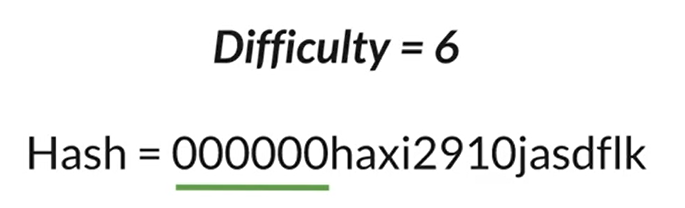
\includegraphics[width=0.5\linewidth]{slike/difficulty.png}
    \caption{Приказ задовољеног хеша}
    \label{fig:good-hash}
\end{figure}

Пронаћи одређени број водећих нула насумично постаје експоненцијално теже како се сама тежина повећава. Дакле, да би се решио доказ рада, рудар ће морати генерисати огроман број хешева како би на крају пронашао један који задовољава тежину. Они ће генерисати нове хешеве за исти блок на основу података блока као и његове прилагођене вредности зване \textit{nonce}.

\subsubsection{\textit{Nonce}}
Променом вредности нонса рудар генерише нове важеће хешеве за текући блок и његове податке. \textit{Nonce} је термин у криптографији који се односи на вредност која се може користити само једном. Пошто свака јединствена вредност \textit{nonce}-a генерише јединствен хеш, \textit{nonce}-i се могу користити само једном за генерисање тог новог хеша за блок.

Вредност нонса почиње од нуле и повећава се док се не пронађе \textit{nonce} који има одговарајући број водећих нула у складу са подешеном тежином, што генерише хеш. Ова вредност \textit{nonce}-a се затим чува као део блока.

\subsubsection{Процес рударења}
Овај процес генерисања нових хешева са променљивим вредностима захтева доста рачунарског рада. Због тога се акт трошења овог рачунарског рада назива рударење. Када рудар успешно ископа блок, они ће поднети свој блок са пронађеном вредношћу нонса осталим рударима.

Када остали рудари сазнају ову вредност нонса, они могу брзо проверити ваљаност тог решења и додати нови блок у ланац. На тај начин, они не морају поново да раде исти рачунарски рад када приме нови блок за додавање у свој \textit{blockchain} и остану ажурни.

\subsubsection{Динамичка тежина додавања блокова}
Са вредношћу \textit{nonce}-a у блоку, имплементирали смо \textit{Proof of work} систем, где рудари морају уложити одређену количину рачунарске снаге како би додали блокове у ланац. Међутим, како се у мрежу \textit{blockchain}-а додаје све више учесника, блокови ће се откривати брже, јер ће постојати већа шанса да бар један рудар пронађе валидан хеш при одређеној тежини. Због тога нам је потребан динамичан систем који прилагођава ниво тежине \textit{blockchain}-а како се у систем додаје све више рудара.

Да бисмо то постигли, можемо додати вредност тежине сваком блоку. Поред тога, такође постављамо временску вредност која представља стопу којом желимо да се сваки блок рудари. Механизам за прилагођавање тежине функционисаће на следећи начин: проверићемо временски жиг ново изрудареног блока и упоредити га са временским жигом претходно изрудареног блока. Ако је разлика између оба временска жига мања од постављене стопе рударења, знамо да је блок изрударен сувише брзо, те ће се тежина повећати за 1. Слично томе, ако је разлика у временским жиговима између нашег најновијег блока и блока који је претходио већа од стопе рударења, знамо да је блок изрударен сувише споро, те ће се тежина смањити за 1. Са овим системом, увек ћемо прилагођавати тежину за сваки блок и требао би имати систем који рудари блокове у одређеним интервалима.


\begin{figure}[h]
    \centering
    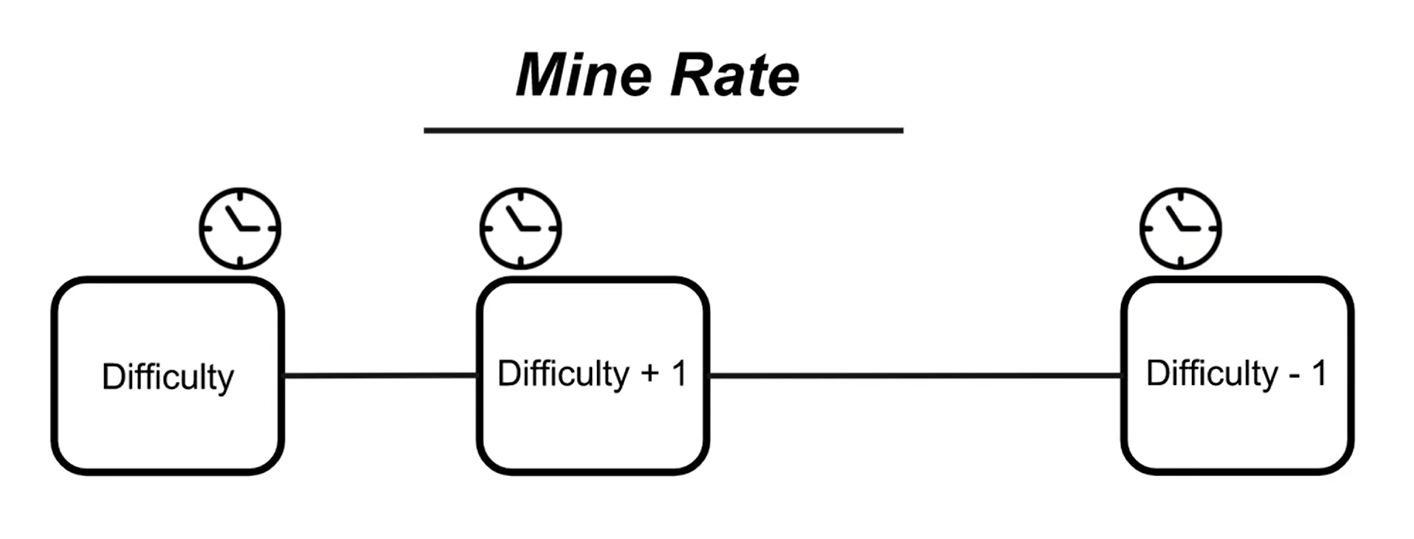
\includegraphics[width=0.7\linewidth]{slike/dynamic-block-difficulty.png}
    \caption{Динамичка промена тежине рударења блока}
    \label{fig:dynamic-mine-rate}
\end{figure}



\subsection{Новчаник и трансакције}
Када проширујемо \textit{blockchain} да укључује криптовалуту, уводимо неколико нових концепата.

\subsubsection{Новчаник}
Дигитални новчаник је повезан са кључевима и трансакцијама. Следећи код приказује структуру новчаника у \textit{Rust} програмском језику:

\begin{minted}{rust}
pub struct Wallet {
    pub balance: u64,
    pub signing_key: SigningKey<Secp256k1>,
    pub verifying_key: VerifyingKey<Secp256k1>,
    pub public_key: String,
}

\end{minted}


Атрибути новчаника су:
\begin{itemize}
    \item \textbf{\textit{balance}}: Стање представља укупну количину валуте која припада појединцу у криптовалутном \textit{blockchain}-у.
    \item \textbf{\textit{signing\_key}}: Приватни кључ користи се за генерисање јединствених дигиталних потписа за сваку трансакцију
    \item \textbf{\textit{verifying\_key}}: Jавни кључ омогућава другима да верификују те потписе.
    \item \textbf{\textit{public\_key}}: Јавна адреса новчаника је иста као и његов јавни кључ, и омогућава другима да шаљу валуту на тај новчаник.
\end{itemize}



\subsubsection{Креирање кључева}
Сваки појединац који жели да обави трансакцију у \textit{blockchain}-у мора потписати податке о трансакцији својим приватним кључем. Потпис се базира на два кључа: приватном, који само корисник има, и јавном, који је свима видљив \cite{11}. Кључеви су јединствени низови бројева који омогућавају кориснику да потпише податке стварањем шифроване хеш вредности. Ова вредност се генерише комбиновањем података о трансакцији и приватног кључа. Свака промена у оригиналним подацима резултује новим потписом.

\subsubsection{Трансакције}
Трансакције представљају размену валуте између два појединца у криптовалутном систему \cite{12}.  Следећи код приказује структуру трансакције у \textit{Rust} програмском језику:

\begin{minted}{rust}
pub struct Transaction {
    pub id: TransactionId,
    pub input: Option<TransactionInput>,
    pub outputs: Vec<TransactionOutput>,
}

pub struct TransactionId(pub Uuid);

\end{minted}

Свака трансакција има два дела: улаз и излаз. 

Улаз трансакције је кључна компонента која описује детаље о извору средстава коришћених у трансакцији. Следећи код приказује структуру улаза трансакције у \textit{Rust} програмском језику:
\begin{minted}{rust}
pub struct TransactionInput {
    pub timestamp: DateTime<Utc>,
    pub amount: u64,
    pub address: String,
    pub signature: String,
}
\end{minted}

Атрибути улаза трансакције су:
\begin{itemize}
    \item \textbf{\textit{timestamp}}: Ово поље представља тачан тренутак када је трансакција креирана. Време је обично записано у \textit{UTC} формату, што омогућава прецизно праћење и синхронизацију у међународним оквирима.
    \item \textbf{\textit{amount}}: Износ представља количину криптовалуте која се преноси са једне адресе на другу. 
    \item \textbf{\textit{address}}: Aдресa представља адресу новчаника са ког средства долазе.
    \item \textbf{\textit{signature}}: Потпис обезбеђује интегритет и аутентичност трансакције
\end{itemize}

Излаз трансакције писује детаље о одредишту средстава која се преносе у трансакцији. Свака трансакција може имати један или више излаза, што омогућава податке о томе где се средства шаљу. У наставку је пример структуре излаза трансакције у програмском језику \textit{Rust}:

\begin{minted}{rust}
pub struct TransactionOutput {
    pub amount: u64,
    pub address: String,
}
\end{minted}

Атрибути излаза трансакције су:
\begin{itemize}
    \item \textbf{\textit{amount}}: Износ представља количину криптовалуте која се преноси на одређену адресу.
    \item \textbf{\textit{address}}: Ова адреса одређује где се средства шаљу.
\end{itemize}

Пример трансакција приказан на слици \ref{fig:transactions-example} илуструје две различите трансакције у \textit{blockchain} мрежи. У првој трансакцији, улаз садржи податке као што су временски печат, баланс од 500 јединица, дигитални потпис и јавни кључ пошиљаоца (0xfoo1). Ова трансакција има два излаза: први излаз преноси 40 јединица на адресу 0xbar2, а други излаз приказује колико ће јединица валуте остати на адреси пошиљаоца (0xfoo1) после извршене трансакције. Ова структура показује како се улазни баланс дели између различитих адреса, где један део иде новом кориснику, а преостали део се враћа пошиљаоцу као кусур.

У другој трансакцији, улаз укључује временски печат, баланс од 300 јединица, дигитални потпис и јавни кључ пошиљаоца (0xzag3). Ова трансакција такође има два излаза: први излаз преноси 20 јединица на адресу 0xfoo1, а други излаз преноси преосталих 280 јединица назад на адресу пошиљаоца (0xzag3). Оваква структура обезбеђује да се трансакције у \textit{blockchain} мрежи извршавају на транспарентан и безбедан начин, чувајући интегритет и прецизност финансијских токова.


\begin{figure}[h]
    \centering
    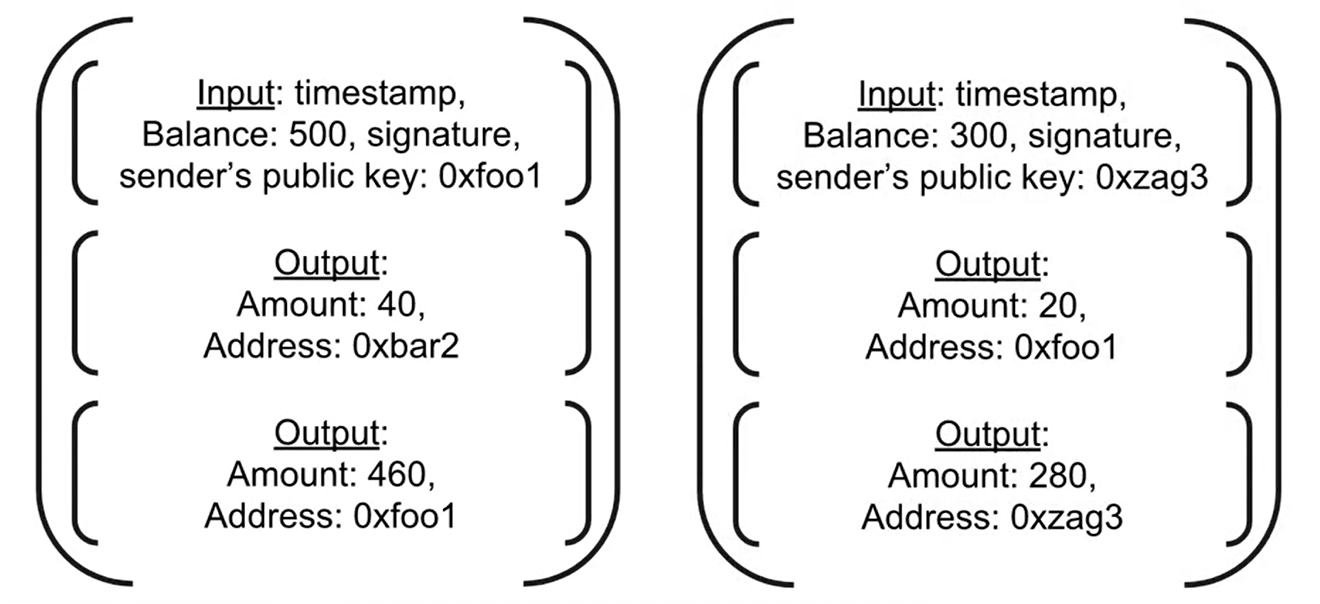
\includegraphics[width=1\linewidth]{slike/transactions-example.png}
    \caption{Пример трансакција}
    \label{fig:transactions-example}
\end{figure}

\subsubsection{Потписивање трансакција}
Свака трансакција мора бити потписана дигиталним потписом корисника. Ово осигурава да подаци нису мењани након потписивања и да потпис одговара јавном кључу пошиљаоца.

\begin{figure}[h]
    \centering
    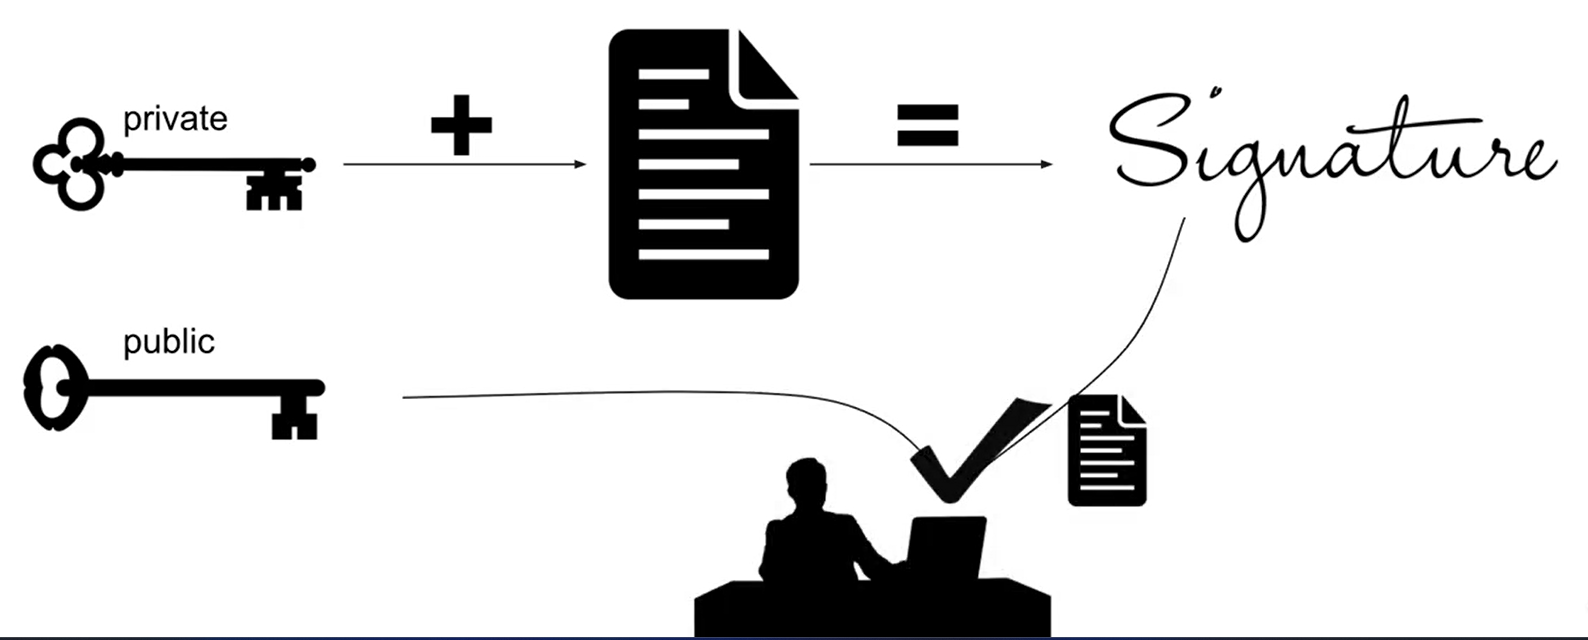
\includegraphics[width=1\linewidth]{slike/signature.png}
    \caption{Дигитални потписи}
    \label{fig:digital-signatures}
\end{figure}

Слика \ref{fig:digital-signatures} илуструје рад приватног и јавног кључа. Приватни кључ је познат само кориснику и служи за стварање потписа, док је јавни кључ доступан свима и користи се за верификацију тог потписа. Ови кључеви су јединствени низови бројева. Корисник потписује податке стварањем потписа који је шифровани хеш вредност. Хеш вредност се генерише комбинацијом података о трансакцији и приватног кључа корисника. Пошто је хеш вредност заснована на оригиналним подацима, свака промена у оригиналним подацима, чак и један знак, резултоваће новом хеш вредношћу и новим потписом.

Сада, када подаци имају потпис, свако може користити јавни кључ корисника који је потписао податке да би верификовао тај потпис. Јавни кључ се користи за дешифровање потписа и читање оригиналних података. Ако дешифровани подаци не одговарају оригиналним подацима из трансакције, знамо да је или оригинални податак измењен након потписивања или је потпис генерисан приватним кључем који не одговара презентованом јавном кључу. У оба случаја, трансакција је неважећа.

\subsubsection{Ажурирање трансакција}
Оптимизација трансакција у \textit{blockchain} систему се може спровести кроз ажурирање постојећих трансакција уместо креирања нових. Овај приступ омогућава бољу ефикасност у управљању трансакцијама и смањује потребу за генерисањем нових објеката за сваку нову трансакцију.

Традиционално, свака трансакција у \textit{blockchain} систему садржи улазне и излазне вредности. Улазна вредност обухвата информације о пошиљаоцу, као што су временска ознака, почетно стање и дигитални потпис. Излазне вредности укључују износ који се шаље и адресу примаоца. Међутим, када појединац жели да обави више трансакција у кратком временском периоду, креирање потпуно нових трансакција може бити неефикасно.

Да би се овај процес оптимизовао, постојеће трансакције се могу проширити са новим излазима који представљају нове размене. На тај начин, један објекат трансакције може садржати више излаза који омогућавају слање валуте на више прималаца. Приликом ажурирања трансакције, потребно је поново потписати трансакцију како би се укључили нови подаци и обезбедила верификација валидности.

Конкретно, сваки нови излаз ће одражавати нову размену валуте, док ће укупни износ свих излаза бити ажуриран да би се одразила нова стања. Овај метод омогућава једноставнију и бржу размену валуте, смањујући потребу за креирањем и управљањем великим бројем трансакцијских објеката.


\begin{figure}[h]
    \centering
    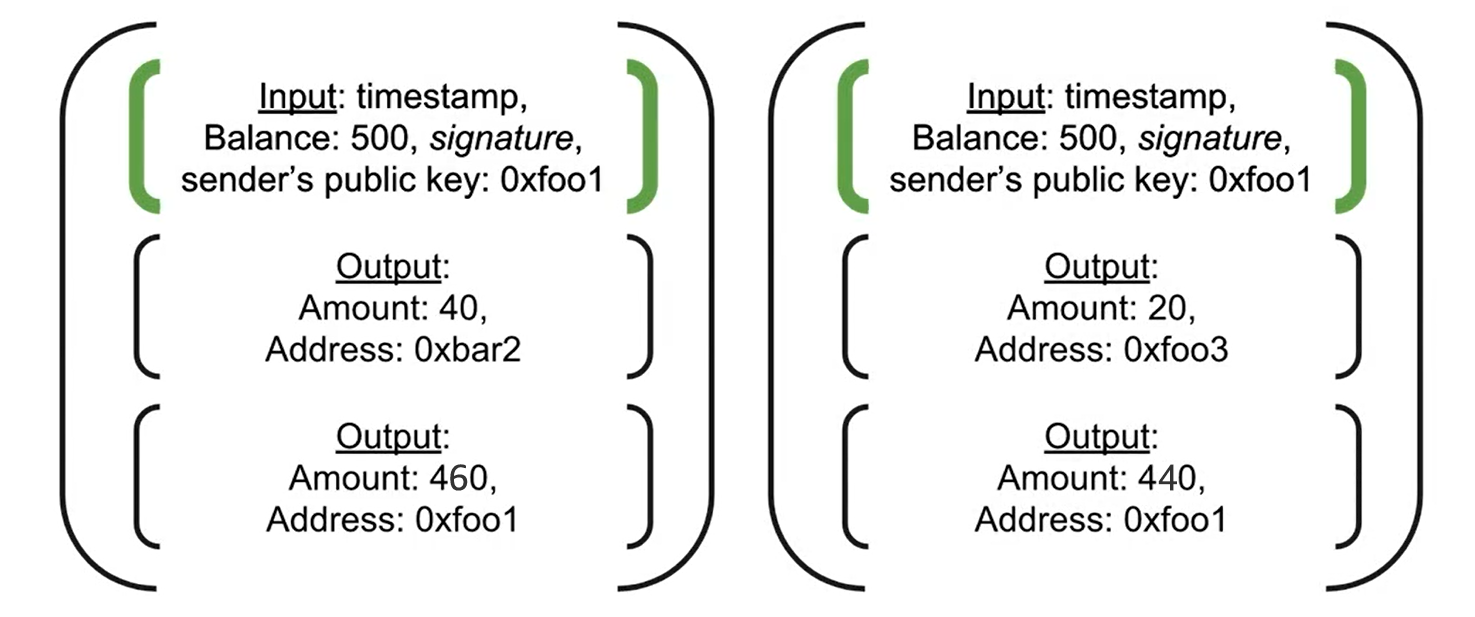
\includegraphics[width=1\linewidth]{slike/transaction-updates-1.png}
    \caption{Пример две трансакције са истим улазом}
    \label{fig:transaction-updates-before}
\end{figure}

\begin{figure}[h]
    \centering
    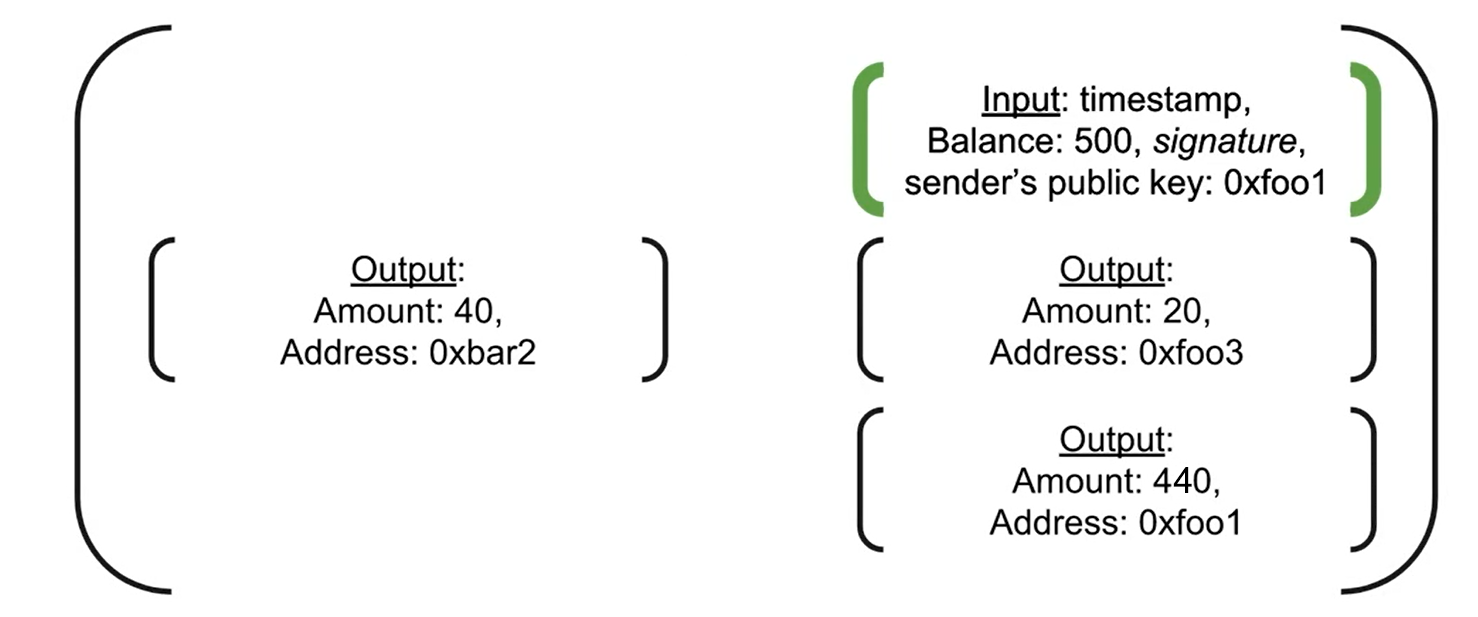
\includegraphics[width=1\linewidth]{slike/transaction-updates-2.png}
    \caption{Пример ажуриране трансакције}
    \label{fig:transaction-updates-now}
\end{figure}


\subsection{Базен трансакција}
Базен трансакција je кључни концепт у \textit{blockchain} технологији који омогућава укључивање група трансакција у блокове. Док више појединаца креира трансакције са својим новчаницима у криптовалутама, потребан је начин да се те трансакције групишу и укључе у \textit{blockchain}. Овај процес се остварује кроз трансакциони базен, који представља објекат који се ажурира у реалном времену и садржи све нове трансакције поднете од стране свих корисника у мрежи криптовалута.

Корисници креирају трансакције једни са другима и подносе их у трансакциони базен. Ове нове трансакције се сматрају непотврђеним јер још увек нису званично укључене у \textit{blockchain}. Рудари имају задатак да креирају блокове који потврђују трансакције тако што узимају групу ових трансакција из базена и укључују их као податке за нови блок у \textit{blockchain}-у. Потврђивање трансакција зависи од брзине којом рудари генеришу нове блокове. Иако се објекти трансакција могу креирати тренутно, постоји кратак период док су непотврђене, све док их рудар не укључи у \textit{blockchain} и тиме их званично потврди.

\begin{figure}[h]
    \centering
    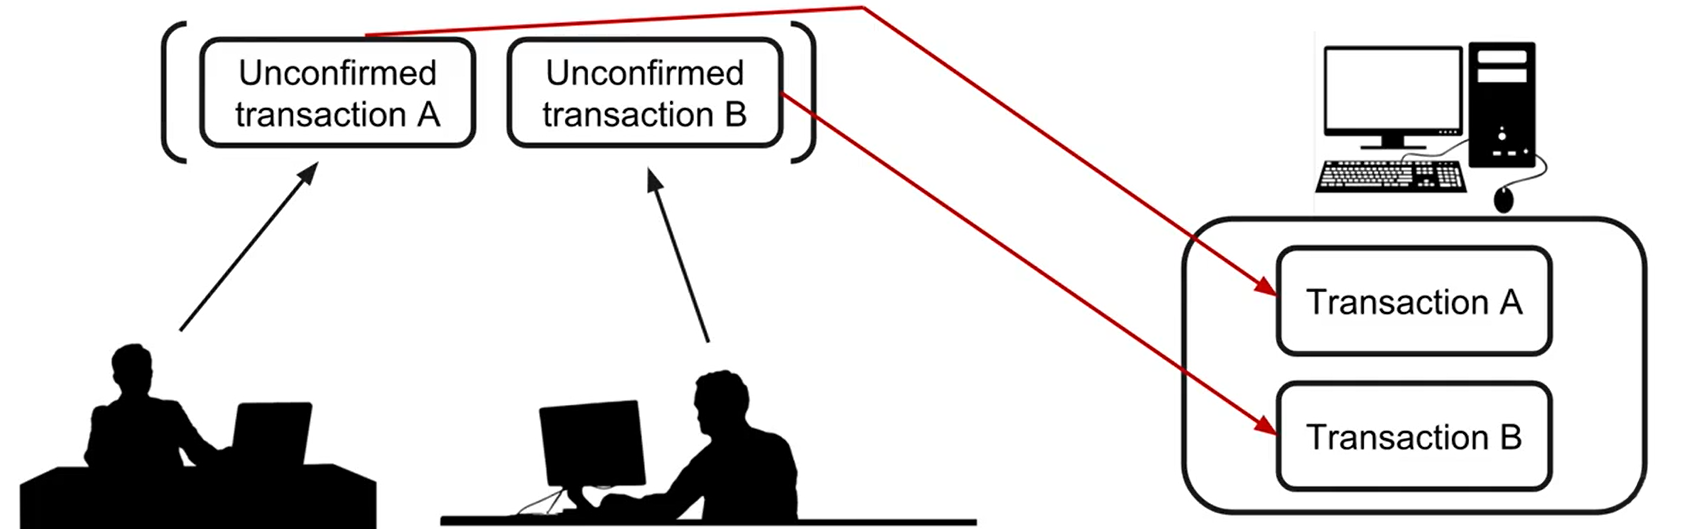
\includegraphics[width=1\linewidth]{slike/transaction-pool.png}
    \caption{Базен трансакција}
    \label{fig:transaction-pool}
\end{figure}

\subsection{Рудари}
Рудари у \textit{blockchain} мрежи играју кључну улогу у обезбеђивању валидности и интегритета трансакција. Када се нова трансакција емитује у мрежу, рудари је проверавају како би се уверили да је валидна. Ово укључује проверу да пошиљалац има довољно средстава, да није покушао да потроши исте јединице два пута (познато као двоструко трошење), као и да је трансакција исправно потписана. Након што рудар верификује трансакцију, додаје је у свој блок трансакција, који потом покушава да дода у \textit{blockchain} кроз процес рударења.

\newpage
\subsubsection{Наградне трансакције}
Наградне трансакције представљају главни подстицај за рударе у \textit{blockchain} мрежама. Када рудар успешно дода нови блок у \textit{blockchain}, добија награду у облику новостворених криптовалута, као и накнаде за трансакције које су укључене у тај блок. Ова награда служи као механизам за увођење нових јединица у циркулацију и подстиче рударе да учествују у одржавању и обезбеђивању мреже \cite{13}. Временом, како број новостворених јединица по блоку опада, накнаде за трансакције постају све значајнији део рударских прихода.

\subsubsection{Пражњење базена трансакција}
Пражњење базена трансакција, познато и као процес уклањања трансакција из базена трансакција, је кључни део рударског процеса. Када рудар успе да дода нови блок у \textit{blockchain}, све валидне трансакције из тог блока се уклањају из базена. Ово обезбеђује да се ове трансакције не обрађују поново и ослобађа простор за нове трансакције које чекају на потврду. Пражњење базена је важно за одржавање ефикасности и брзине мреже, јер спречава загушење и омогућава рударима да фокусирају своје ресурсе на обраду нових трансакција.

\subsubsection{Стање новчаника}
Са трансакцијама сачуваним на \textit{blockchain}-у, корисници могу израчунати своје стање у валути на основу историје \textit{blockchain}-а. Основна идеја је да збир свих излазних трансакција у сваком блоку, које су адресиране на јавни кључ корисника, представља укупно стање његовог рачуна.

Поставља се питање када желимо ажурирати ово стање. Приликом сваке трансакције, вршимо размену валуте на основу тренутног стања корисника. Стога је најбоље израчунати ово стање за сваки кориснички новчаник када год се обави нека трансакција. 

Основна идеја за израчунавање стања је да се саберу сви излази који припадају појединцу. Међутим, рачуница може бити мало сложенија. Постоји једна замка. Наиме, стање корисника је збир свих излаза који му припадају, али је то само збир свих трансакција од последње трансакције коју је тај корисник обавио. Ако корисник обави трансакцију, генерише се излаз који показује колико валуте треба да му остане након трансакције. Следеће рачунање стања може користити овај излаз, као и било које претходне износе, што би било двоструко бројање трансакција у историји стања корисника.

\begin{figure}[h]
    \centering
    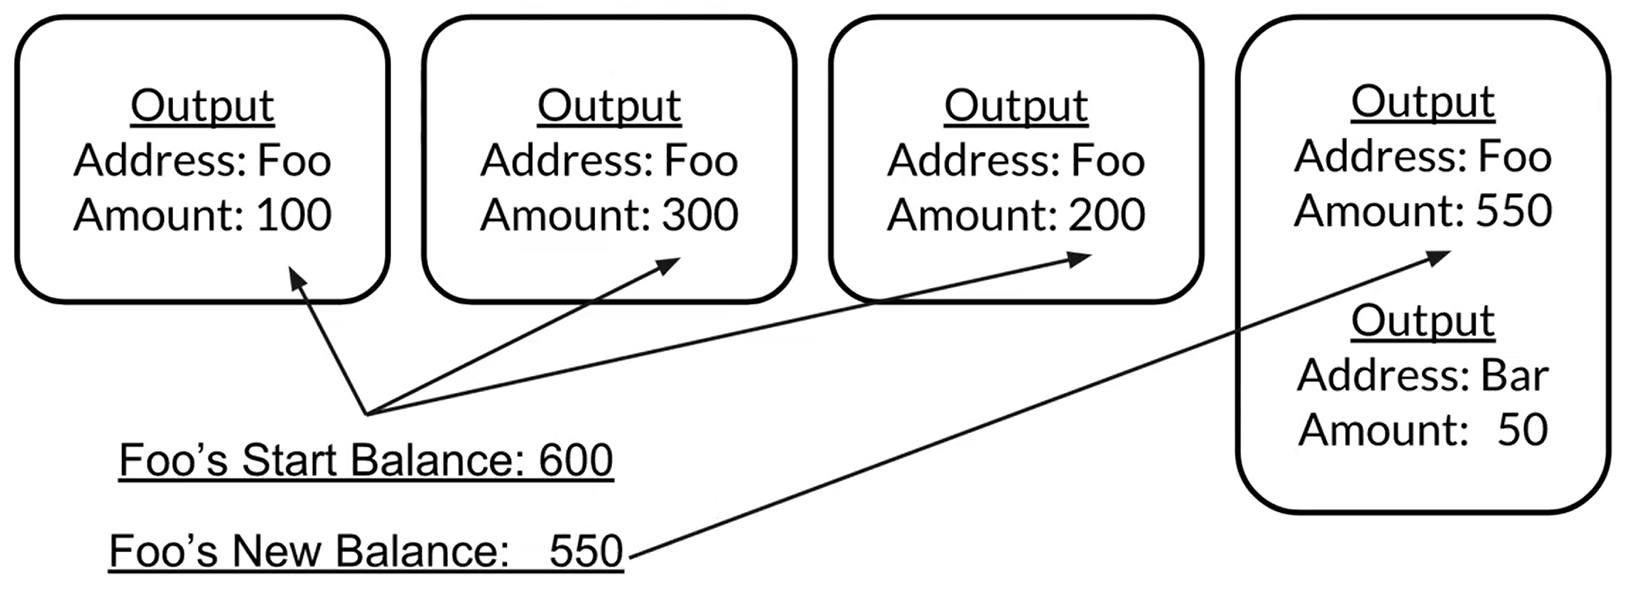
\includegraphics[width=1\linewidth]{slike/balance.png}
    \caption{Пример рачунања стања}
    \label{fig:balance}
\end{figure}
\pagebreak
Размотримо овај могући проблем на примеру са слике \ref{fig:balance}. Рецимо да корисник \textit{Foo} жели да обави трансакцију и пошаље валуту кориснику \textit{Bar}. \textit{Foo}-ово стање се поново израчунава сабирањем свих излаза у историји \textit{blockchain}-а који су му послали валуту. \textit{Foo}-ово стање је израчунато као 600 на основу претходних трансакција. Када се нова \textit{Foo}-ова трансакција, у којој шаље 50 \textit{Bar}-у, дода у \textit{blockchain}, нова трансакција приказује да је 50 \textit{Foo}-ових валута послато \textit{Bar}-у, остављајући \textit{Foo}-у 550 валута. Стога, \textit{Foo}-ово стање би требало да буде 550. Али ако поновно рачунање стања сабере све излазе у историји \textit{blockchain}-а, стање ће заправо бити 600 плус 550, што је 1150 и није тачно.

Дакле, право стање корисника се израчунава само сабирањем излаза који су настали од последње трансакције тог корисника, укључујући и ту последњу трансакцију. Стога, рачунање стања које гледа само на најновију трансакцију и било које наредне излазе приказује право стање за тог корисника. У овом случају, право стање \textit{Foo}-а је 550.


\newpage
\subsection{Класни дијаграм архитектуре \textit{blockchain} мреже}

\begin{figure}[h]
    \centering
    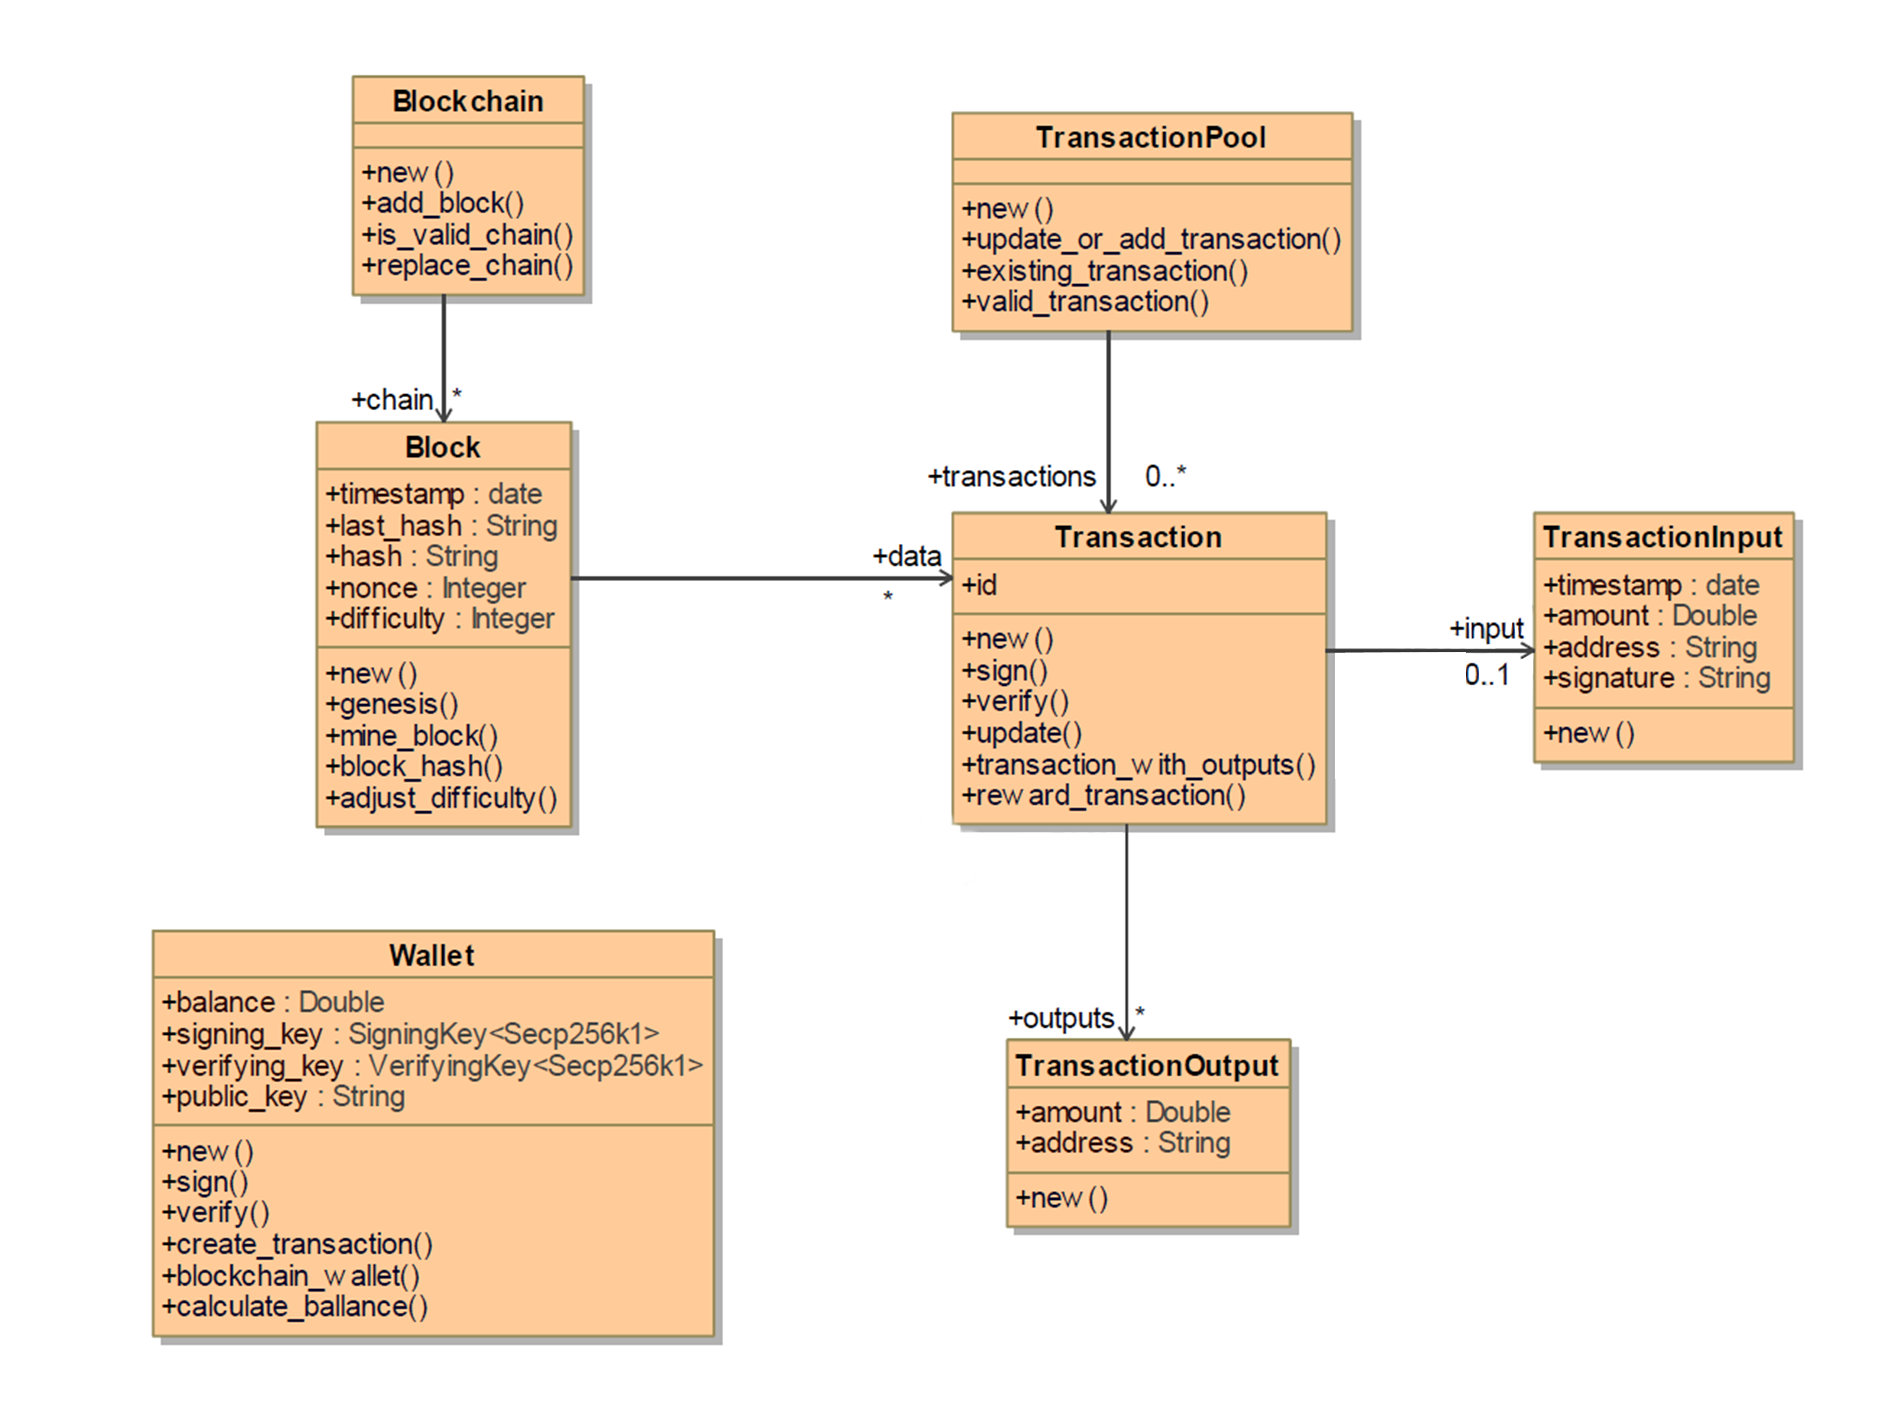
\includegraphics[width=1\linewidth]{slike/blockchain_class.png}
    \caption{Класни дијаграм архитектуре \textit{blockchain} мреже}
    \label{fig:enter-label}
\end{figure}

\newpage



\section{\textit{Blockchain} клијенти - чворови}
Чворови (\textit{Nodes}) су основни елементи \textit{P2P} мрежа који омогућавају комуникацију и размену података између корисника. Они одржавају копије \textit{blockchain}-a, управљају трансакцијама и осигуравају интегритет и безбедност мреже. Чворови такође обрађују и верификују трансакције, доприносећи децентрализацији и поузданости система. Следећи код у \textit{Rust}-у приказује структуру једног чвора:

\begin{minted}{rust}
pub struct Node{
    pub blockchain: Arc<RwLock<Blockchain>>,
    pub host_port: String,
    pub event_sender: Option<mpsc::Sender<String>>,
    pub wallet: Arc<RwLock<Wallet>>,
    pub transaction_pool: Arc<RwLock<TransactionPool>>
}

\end{minted}

Атрибути чвора су:
\begin{itemize}
    \item \textbf{\textit{blockchain}}: Ово поље представља \textit{blockchain} који чвор одржава. Користи се \textit{Arc\footnotemark{1}<RwLock\footnotemark{2}<Blockchain>>} за омогућавање сигурног приступа \textit{blockchain}-у из више нитова, обезбеђујући истовремени приступ без конфликта.
    \item \textbf{\textit{host\_port}}: Овај атрибут чува информације о порту на којем чвор слуша за долазне везе. Формат је \textit{String}, који омогућава лако конфигурисање и читање из подешавања.
    \item \textbf{\textit{event\_sender}}: Пошиљалац догађаја је опциони атрибут \linebreak(\textit{Option<mpsc::Sender<String>>}) који омогућава слање догађаја другим компонентама система. Користи се за међусобну комуникацију унутар чвора.
    \item \textbf{\textit{wallet}}: Новчаник чвора који чува криптовалуте и кључеве. Користи се \linebreak\textit{Arc<RwLock<Wallet>>} за истовремени приступ из више нитова, обезбеђујући сигурност и интегритет података.
    \item \textbf{\textit{transaction\_pool}}: Базен трансакција који чвор одржава. Ово поље \linebreak(\textit{Arc<RwLock<TransactionPool>>}) омогућава складиштење и приступ тренутним трансакцијама које чекају да буду додане у \textit{blockchain}.
\end{itemize}
\footnotetext[1]{\textit{Arc (Atomic Reference Counted)} је структура у програмском језику \textit{Rust} која омогућава сигурно дељење података између више нитова. Користи атомски бројач референци да би осигурала да ће подаци бити ослобођени када више не буде референци на њих \cite{6}.}
\footnotetext[2]{\textit{RwLock (Read-Write Lock)} је механизам закључавања који омогућава више читалаца да истовремено приступају подацима, али само један писач може да приступа подацима у истом тренутку. Омогућава ефикасно управљање приступом разликовањем читања од писања \cite{6}.}
\newpage
Приликом покретања апликације прослеђује се порт за \textit{http} сервер, иницијализује се и покреће чвор. Покретање се врши следећом функцијом:

\begin{minted}{rust}
impl Node {
    pub async fn start(mut self) -> Result<(), Box<dyn std::error::Error>>{
        let (event_sender, event_receiver) = mpsc::channel(100);
        self.event_sender = Some(event_sender.clone());
        let swarm = build_swarm()?;
        let p2p = subscribe(self.clone(), event_receiver, swarm);
        let http = run_server(self.clone());
        _ = tokio::join!(p2p, http);
        Ok(())
    }
}
\end{minted}

Приликом покретања чвора се иницијализује асинхрони канал који служи за пренос порука између \textit{http} i \textit{p2p} сервера. Затим се иницијализују \textit{http} i \textit{p2p} сервери и покрећу у асинхроним задацима.

\subsection{\textit{P2P} сервер}
Комуникација између чворова у дистрибуираним системима је од суштинског значаја за функционисање \textit{blockchain} мрежа.
Понашање мреже дефинише како чворови комуницирају једни са другима. У овом случају коришћени су \textit{gossipsub} за емитовање порука и \textit{mdns} за откривање других чворова.

\begin{minted}{rust}
#[derive(NetworkBehaviour)]
pub(crate) struct MyBehaviour {
    pub(crate) gossipsub: gossipsub::Behaviour,
    mdns: mdns::tokio::Behaviour,
}
\end{minted}

Чворови су подешени да ове поруке очекују на различитим мрежним протоколима и портовима.

\begin{minted}{rust}
swarm.listen_on("/ip4/0.0.0.0/udp/0/quic-v1".parse()?)?;
swarm.listen_on("/ip4/0.0.0.0/tcp/0".parse()?)?;
\end{minted}

\newpage
Ове линије кода омогућавају чвору да прихвата долазне мрежне везе на било којој доступној \textit{IPv4}\footnotemark[1] адреси, користећи аутоматски додељене портове за оба \textit{UDP}\footnotemark[2] (са \textit{QUIC}\footnotemark[3] протоколом) и \textit{TCP}\footnotemark[4]. Ова конфигурација осигурава да чвор може да комуницира са другим чворовима у мрежи путем различитих мрежних протокола, обезбеђујући флексибилност и компатибилност.

\footnotetext[1]{\textit{IPv4 (Internet Protocol version 4)} је протокол који дефинише начин на који се подаци преносе унутар мреже и између мрежа на Интернету. Користи 32-битне адресе, што омогућава приближно 4 милијарде јединствених адреса \cite{14}.}

\footnotetext[2]{\textit{UDP (User Datagram Protocol)} је протокол који омогућава брз и лаган пренос података без успостављања везе. За разлику од \textit{TCP}-а, не гарантује поузданост или редослед преноса података, али је погодан за апликације где је брзина важнија од поузданости \cite{15}.}

\footnotetext[3]{\textit{QUIC (Quick UDP Internet Connections)} је протокол који побољшава брзину и безбедност интернет комуникација. Користи \textit{UDP} као основу и интегрише функције које су типичне за \textit{TCP} и \textit{TLS} \textit{(Transport Layer Security)}. Омогућава брже успостављање везе и смањује латентност, док истовремено пружа унапредену безбедност \cite{16}.}

\footnotetext[4]{\textit{TCP (Transmission Control Protocol)} је протокол који осигурава поуздано и уређено преношење података између рачунара у мрежи. Он успоставља везу пре преноса података и гарантује да ће сви подаци стићи у исправном редоследу \cite{15}.}








Чворови се претплаћују на различите теме и обрађују догађаје који се појављују на мрежи. Ово укључује слушање на одређеним адресама и обраду порука које се примају. Три теме које чворови прате су:
\begin{enumerate}
    \item \textbf{\textit{blockchain}}
    \item \textbf{\textit{transaction\_pool}}
    \item \textbf{\textit{transaction\_pool\_clear}}
    
\end{enumerate}

\subsubsection{\textbf{\textit{blockchain}} тема}
Тема \textit{blockchain} служи за размену података о стању ланца блокова између чворова у мрежи. Ово укључује слање и примање ажурирања о новом блоку који је додат у ланац. Ово омогућава свим чворовима у мрежи да буду синхронизовани и имају ажурирани ланац блокова.

Када чвор креира нови блок, он шаље поруку свим претплаћеним чворовима са информацијама о новом блоку. Ова порука укључује комплетан ланац блокова. Када чвор прими поруку о ланцу блокова, он упоређује примљени ланац са својим тренутним ланцем. Ако је примљени ланац дужи и ваљан, чвор ажурира свој ланац новим блоковима. Ово обезбеђује да сви чворови имају најдужи и најновији ланац блокова.

\newpage
\subsubsection{\textbf{\textit{transaction\_pool}} тема}
Тема \textit{transaction\_pool} служи за размену трансакција које чекају да буду укључене у нови блок. Ово омогућава чворовима да деле непотврђене трансакције и осигурава да су све валидне трансакције на располагању за рударење. Ово омогућава да све трансакције буду видљиве и доступне свим чворовима у мрежи.

Када чвор креира нову трансакцију, он шаље поруку свим претплаћеним чворовима са информацијама о новој трансакцији. Ова порука укључује детаље о трансакцији. Када чвор прими поруку о новој трансакцији, он проверава валидност трансакције. Ако је трансакција валидна, додаје је у свој базен трансакција, чиме се обезбеђује да све важеће трансакције буду доступне за рударење у следећем блоку. Ако трансакција са истим пошиљаоцем већ постоји у базену, ажурира се постојећа трансакција тако што јој се додаје излаз нове трансакције у листу излаза.


\subsubsection{\textbf{\textit{transaction\_pool\_cleer}} тема}
Тема \textit{transaction\_pool\_clear} служи за чишћење базена трансакција. Ово се користи када је нови блок креиран и све укључене трансакције треба да буду уклоњене из базена трансакција како би се избегле дуплиране трансакције. Ово обезбеђује да базен трансакција буде ажуриран и да укључује само непотврђене трансакције.

Када чвор креира нови блок и укључи трансакције из базена трансакција у тај блок, он шаље поруку свим претплаћеним чворовима са захтевом да очисте свој базен трансакција. Ова порука може укључивати списак трансакција које су укључене у нови блок.
Када чвор прими поруку о чишћењу базена трансакција, он уклања све трансакције које су укључене у нови блок из свог базена трансакција. Ово осигурава да базен трансакција садржи само трансакције које још нису укључене у \textit{blockchain}.
\newpage
\subsection{\textit{HTTP} сервер}
\textit{HTTP} сервер за \textit{blockchain} клијента је веб сервер који пружа интерфејс за комуникацију са \textit{blockchain} мрежом преко \textit{HTTP} протокола. Овај сервер омогућава корисницима и другим апликацијама да интеракцију са \textit{blockchain}-ом мрежом путем различитих \textit{endpoint}-ова, што укључује прегледивање \textit{blockchain}-а, вршење трансакција и управљање новчаником.

Сервер користи асинхроне функције које омогућавају ефикасно руковање \textit{HTTP} захтевима без блокирања. Функције користе \textit{await} за чекање на резултате асинхроних операција као што су закључавање \textit{mutex}-а или читање података из \textit{blockchain}-а. Пример једне функције је дат у коду који следи:

\begin{minted}[breaklines]{rust}
pub async fn get_wallet_balance(node: Arc<Mutex<Node>>) -> Result<impl warp::Reply, warp::Rejection> {
    let node = node.lock().await;
    let wallet = node.wallet.read().await.clone();
    let blockchain = node.blockchain.read().await.clone();
    let balance = wallet.calculate_balance(&blockchain);
    Ok(warp::reply::with_status(warp::reply::json(&balance), StatusCode::OK))
}
\end{minted}

Да бисмо у сваки \textit{HTTP} захтев додали копију објекта чвора морамо направити одговарајући филтер. \textit{warp::any()} ствара филтер који прихвата све захтеве без додатних услова, док метод \textit{map(move || node.clone())} дефинише анонимну функцију која враћа копију \textit{node}. Кључна реч \textit{move} осигурава да затвор преузме власништво над \textit{node}, што омогућава сигурно коришћење \textit{node} у асинхроним функцијама. Овај филтер омогућава рутама да приступе \textit{node} објекту, који може бити дељен и коришћен за различите операције унутар \textit{HTTP} сервера. Код је приказан испод:

\begin{minted}{rust}
    let node_filter = warp::any().map(move || node.clone());
\end{minted}


\textit{Warp} користи филтере за дефинисање рута и обраду захтева. Свакa рута (\textit{/blockchain, /mine, /transaction}, итд.) је дефинисана помоћу комбинaција \textit{warp::get(),\newline warp::post()}, и других метода за спецификацију \textit{HTTP} метода и путања. Филтери омогућавају повезивање руте са одговарајућим асинхроним функцијама које обрађују захтеве. Пример једног таквог захтева је у коду који следи:

\begin{minted}[breaklines]{rust}
let wallet_balance = warp::get()
        .and(warp::path("balance"))
        .and(warp::path::end())
        .and(node_filter.clone())
        .and_then(routes::get_wallet_balance);
\end{minted}


\textit{CORS (Cross-Origin Resource Sharing)} је конфигурисан путем \textit{warp::cors()} како би се омогућио приступ серверу из различитих извора. Ово је посебно важно за клијенте који се налазе на различитим доменима или портовима. 

\begin{minted}[breaklines]{rust}
let cors = warp::cors()
        .allow_any_origin()
        .allow_header("content-type")
        .allow_methods(&[
            Method::PUT,
            Method::DELETE,
            Method::GET,
            Method::POST,
        ]);

\end{minted}


Руте се конфигуришу тако што \textit{Warp} спаја различите филтере који одговарају на различите врсте захтева. Почиње са основним рутом а затим користи метод \textit{or} за додавање додатних рута. Метод \textit{or} омогућава да се свака рутa додатно обрађује ако претходна рутa не одговара на захтев. Након дефинисања рутa, код додаје \textit{CORS} конфигурацију помоћу \textit{.with(cors)}, што омогућава захтеве из различитих извора, и укључује праћење захтева користећи \textit{.with(warp::trace::request())} за записивање информација о свим \textit{HTTP} захтевима, што помаже у дебаговању и надзору.

\begin{minted}[breaklines]{rust}
hello
    .or(blockchain)
    .or(mine_block)
    .or(print_transactions)
    .or(post_transaction)
    .or(public_key)
    .or(wallet_balance)
    .with(cors)
    .with(warp::trace::request())
\end{minted}

Функција \textit{run\_server} користи \textit{warp::serve()} за покретање сервера на специфичној \textit{IP} адреси и порту. \textit{IP} адреса [0, 0, 0, 0] значи да сервер слуша на свим доступним мрежним интерфејсима, док се порт преузима из конфигурације објекта чвора.

\begin{minted}[breaklines]{rust}
let host_port: u16 = node.lock().await.host_port.parse().unwrap();
warp::serve(routes).run(([0, 0, 0, 0], host_port)).await;
\end{minted}

\newpage
\section{Ограничења и унапређења}
\textit{Blockchain} системи имају нека значајна ограничења. Једно од главних ограничења је скала. Наиме, свако \textit{blockchain} решење може бити ограничено у броју трансакција које може обрадити у одређеном временском периоду, што може довести до кашњења у обради и повећања трошкова трансакција. 

Такође, процес \textit{mining}-а захтева велики број рачунарских ресурса, што може довести до високе потрошње енергије и потребе за специјализованим хардвером.

Поред тога, процес синхронизације и распрострањивања блокова између различитих чворова у мрежи може бити спор и сложен, посебно у великим системима. Иако \textit{blockchain} нуди висок ниво безбедности, постоје и ризици као што су напади 51\% или слаба сигурност приватних кључева.

Како би се превазишла ова ограничења, могу се размотрити различита унапређења. Једна од могућности је увођење трансакционих такси, које би могле проценат валуте по свакој трансакцији. Ове таксе не само да помажу у покривању трошкова операције, већ могу и побољшати подстицаје за мајнере, јер би део такси био укључен у награду мајнера који пронађе нови блок.

Друга могућност је унапређење функције \textit{mine()} тако што ће обрађивати само групу трансакција из базена трансакција, а не цео базен. Ово би могло побољшати ефикасност и смањити време потребно за обраду свих трансакција.

Коначно, усмеравање трансакција које одобрава \textit{blockchain} кроз посебан сервер могло би повећати безбедност и смањити ризик од злоупотреба, пошто неће сви моћи да праве трансакције путем специјализованог \textit{blockchain} новчаника. ж

Такође, постепено смањење награде за \textit{mining} може помоћи у одржавању дугорочне одрживости система и смањењу инфлације валуте, што је честа пракса у многим криптовалутама.


\newpage
\section{Закључак}
У овом раду представљен је процес дизајна и имплементације \textit{blockchain} система. Почетни део рада обухвата теоретске основе \textit{blockchain} технологије, укључујући основне концепте као што су блокови, ланац, и процес рударења. Описани су принципи функционисања блокова, методе валидизације и начини обраде трансакција у мрежи, као и важне компоненте попут хеш функција и доказ рада.

Такође, имплементација \textit{P2P} сервера који омогућава комуникацију између чворова у мрежи представљена је у раду. Овај сервер обрађује и синхронизује податке између различитих чворова, омогућавајући тако дисеминацију информација и одржавање интегритета \textit{blockchain} података у целој мрежи.

Поред тога, описана је и имплементација \textit{HTTP} сервера који служи за комуникацију са корисничким интерфејсом. Овај сервер обрађује захтеве за приказ \textit{blockchain}, рударење блокова, и управљање трансакцијама. Његова улога је да омогући корисницима да приступе функцијама система и управљају трансакцијама у оквиру \textit{blockchain} мреже.

На крају, указана су и могућа ограничења тренутног система, као и предлози за његово унапређење. Ограничења се односе на скалабилност, ресурсе, и безбедност, док предложена унапређења укључују увођење трансакционих такси, развој напредног корисничког интерфејса, и оптимизацију функције мајнинг-а. Ове измене могле би побољшати перформансе и функционалност \textit{blockchain} система.

Рад пружа увид у креирање и имплементацију \textit{blockchain} система, иако има и простора за додатно усавршавање. Анализа и предложена унапређења могу бити корисне за будући развој и побољшање \textit{blockchain} технологије.


\pagebreak
\section{Литература}
\renewcommand{\refname}{}
\vspace{-\parskip} % Remove extra space added by \parskips
\vspace{-\parskip} % Remove extra space added by \parskips
\vspace{-\parskip} % Remove extra space added by \parskips
\vspace{-\parskip} % Remove extra space added by \parskips
\setlength{\bibsep}{8pt}
\bibliography{bibliography}


\pagebreak
\section{Подаци о кандидату}
Кандидат Бојан Мијановић је рођен 2002. године у Зрењанину. Завршио је средњу школу у Зрењанину, 2020. године као ђак генерације. Факултет Техничких Наука у Новом Саду је уписао 2020. године. Испунио је све обавезе и положио је све испите предвиђеним студијским програмом са просечном оценом од 9.75.


\end{document}

